% Created by tikzDevice version 0.12
% !TEX encoding = UTF-8 Unicode
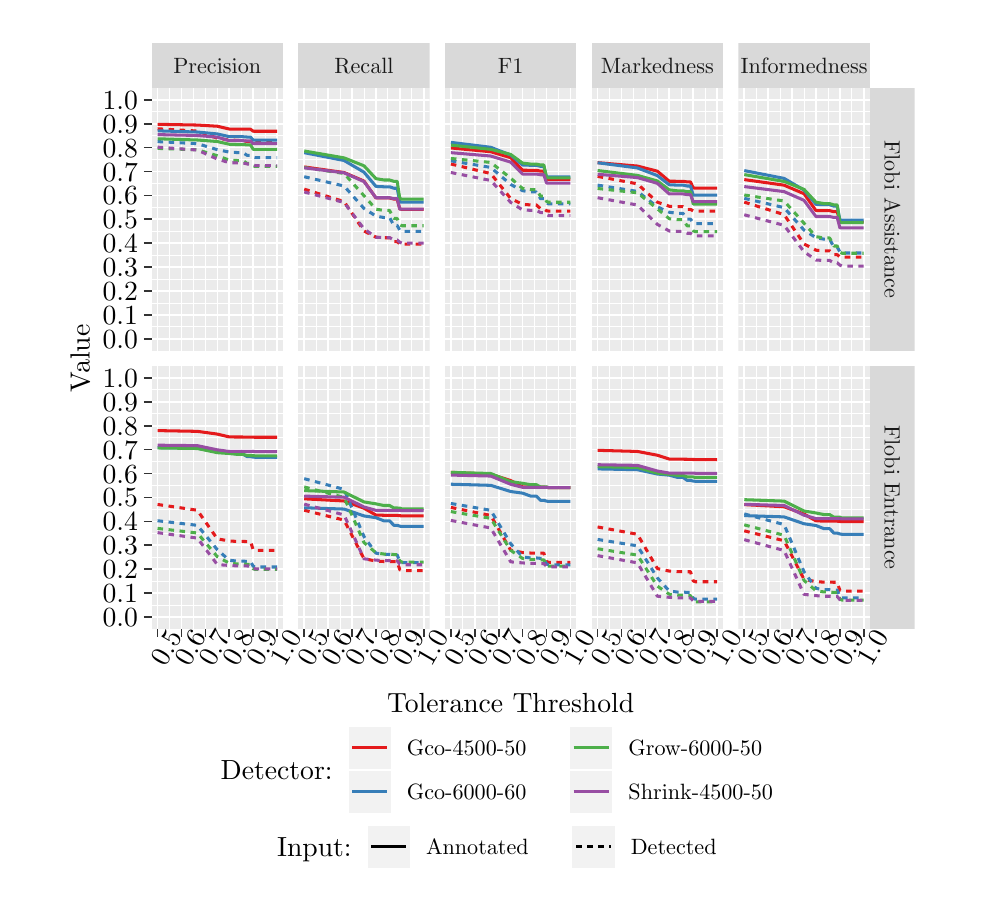
\begin{tikzpicture}[x=1pt,y=1pt]
\definecolor{fillColor}{RGB}{255,255,255}
\path[use as bounding box,fill=fillColor,fill opacity=0.00] (0,0) rectangle (336.00,311.47);
\begin{scope}
\path[clip] (  9.96,  0.00) rectangle (326.04,311.47);
\definecolor{drawColor}{RGB}{255,255,255}
\definecolor{fillColor}{RGB}{255,255,255}

\path[draw=drawColor,line width= 0.6pt,line join=round,line cap=round,fill=fillColor] (  9.96,  0.00) rectangle (326.04,311.47);
\end{scope}
\begin{scope}
\path[clip] ( 44.77,194.71) rectangle ( 92.27,289.72);
\definecolor{fillColor}{gray}{0.92}

\path[fill=fillColor] ( 44.77,194.71) rectangle ( 92.27,289.72);
\definecolor{drawColor}{RGB}{255,255,255}

\path[draw=drawColor,line width= 0.3pt,line join=round] ( 44.77,203.35) --
	( 92.27,203.35);

\path[draw=drawColor,line width= 0.3pt,line join=round] ( 44.77,211.99) --
	( 92.27,211.99);

\path[draw=drawColor,line width= 0.3pt,line join=round] ( 44.77,220.62) --
	( 92.27,220.62);

\path[draw=drawColor,line width= 0.3pt,line join=round] ( 44.77,229.26) --
	( 92.27,229.26);

\path[draw=drawColor,line width= 0.3pt,line join=round] ( 44.77,237.90) --
	( 92.27,237.90);

\path[draw=drawColor,line width= 0.3pt,line join=round] ( 44.77,246.53) --
	( 92.27,246.53);

\path[draw=drawColor,line width= 0.3pt,line join=round] ( 44.77,255.17) --
	( 92.27,255.17);

\path[draw=drawColor,line width= 0.3pt,line join=round] ( 44.77,263.81) --
	( 92.27,263.81);

\path[draw=drawColor,line width= 0.3pt,line join=round] ( 44.77,272.44) --
	( 92.27,272.44);

\path[draw=drawColor,line width= 0.3pt,line join=round] ( 44.77,281.08) --
	( 92.27,281.08);

\path[draw=drawColor,line width= 0.3pt,line join=round] ( 51.25,194.71) --
	( 51.25,289.72);

\path[draw=drawColor,line width= 0.3pt,line join=round] ( 55.57,194.71) --
	( 55.57,289.72);

\path[draw=drawColor,line width= 0.3pt,line join=round] ( 59.88,194.71) --
	( 59.88,289.72);

\path[draw=drawColor,line width= 0.3pt,line join=round] ( 64.20,194.71) --
	( 64.20,289.72);

\path[draw=drawColor,line width= 0.3pt,line join=round] ( 68.52,194.71) --
	( 68.52,289.72);

\path[draw=drawColor,line width= 0.3pt,line join=round] ( 77.16,194.71) --
	( 77.16,289.72);

\path[draw=drawColor,line width= 0.3pt,line join=round] ( 85.79,194.71) --
	( 85.79,289.72);

\path[draw=drawColor,line width= 0.6pt,line join=round] ( 44.77,199.03) --
	( 92.27,199.03);

\path[draw=drawColor,line width= 0.6pt,line join=round] ( 44.77,207.67) --
	( 92.27,207.67);

\path[draw=drawColor,line width= 0.6pt,line join=round] ( 44.77,216.31) --
	( 92.27,216.31);

\path[draw=drawColor,line width= 0.6pt,line join=round] ( 44.77,224.94) --
	( 92.27,224.94);

\path[draw=drawColor,line width= 0.6pt,line join=round] ( 44.77,233.58) --
	( 92.27,233.58);

\path[draw=drawColor,line width= 0.6pt,line join=round] ( 44.77,242.22) --
	( 92.27,242.22);

\path[draw=drawColor,line width= 0.6pt,line join=round] ( 44.77,250.85) --
	( 92.27,250.85);

\path[draw=drawColor,line width= 0.6pt,line join=round] ( 44.77,259.49) --
	( 92.27,259.49);

\path[draw=drawColor,line width= 0.6pt,line join=round] ( 44.77,268.13) --
	( 92.27,268.13);

\path[draw=drawColor,line width= 0.6pt,line join=round] ( 44.77,276.76) --
	( 92.27,276.76);

\path[draw=drawColor,line width= 0.6pt,line join=round] ( 44.77,285.40) --
	( 92.27,285.40);

\path[draw=drawColor,line width= 0.6pt,line join=round] ( 46.93,194.71) --
	( 46.93,289.72);

\path[draw=drawColor,line width= 0.6pt,line join=round] ( 55.57,194.71) --
	( 55.57,289.72);

\path[draw=drawColor,line width= 0.6pt,line join=round] ( 64.20,194.71) --
	( 64.20,289.72);

\path[draw=drawColor,line width= 0.6pt,line join=round] ( 72.84,194.71) --
	( 72.84,289.72);

\path[draw=drawColor,line width= 0.6pt,line join=round] ( 81.48,194.71) --
	( 81.48,289.72);

\path[draw=drawColor,line width= 0.6pt,line join=round] ( 90.11,194.71) --
	( 90.11,289.72);
\definecolor{drawColor}{RGB}{228,26,28}

\path[draw=drawColor,line width= 1.1pt,line join=round] ( 46.93,276.55) --
	( 61.32,276.28) --
	( 68.52,275.85) --
	( 72.84,274.84) --
	( 75.72,274.84) --
	( 77.77,274.84) --
	( 79.32,274.77) --
	( 80.52,274.77) --
	( 81.48,274.05) --
	( 82.26,274.04) --
	( 82.92,274.04) --
	( 90.10,274.04);

\path[draw=drawColor,line width= 1.1pt,dash pattern=on 2pt off 2pt ,line join=round] ( 46.93,274.94) --
	( 61.32,274.11) --
	( 68.52,271.53) --
	( 72.84,270.83) --
	( 75.72,270.76) --
	( 77.77,270.76) --
	( 79.32,270.27) --
	( 80.52,270.27) --
	( 81.48,269.99) --
	( 82.26,269.95) --
	( 82.92,269.95) --
	( 90.10,269.95);
\definecolor{drawColor}{RGB}{55,126,184}

\path[draw=drawColor,line width= 1.1pt,line join=round] ( 46.93,274.19) --
	( 61.32,273.76) --
	( 68.52,273.07) --
	( 72.84,272.09) --
	( 75.72,272.06) --
	( 77.77,272.06) --
	( 79.32,271.95) --
	( 80.52,271.95) --
	( 81.48,270.83) --
	( 82.26,270.82) --
	( 82.92,270.82) --
	( 90.10,270.82);

\path[draw=drawColor,line width= 1.1pt,dash pattern=on 2pt off 2pt ,line join=round] ( 46.93,270.30) --
	( 61.32,269.55) --
	( 68.52,267.39) --
	( 72.84,266.52) --
	( 75.72,266.34) --
	( 77.77,266.34) --
	( 79.32,265.31) --
	( 80.52,265.31) --
	( 81.48,264.64) --
	( 82.26,264.48) --
	( 82.92,264.48) --
	( 90.10,264.48);
\definecolor{drawColor}{RGB}{77,175,74}

\path[draw=drawColor,line width= 1.1pt,line join=round] ( 46.93,271.32) --
	( 61.32,270.88) --
	( 68.52,270.33) --
	( 72.84,269.34) --
	( 75.72,269.23) --
	( 77.77,269.23) --
	( 79.32,269.12) --
	( 80.52,269.12) --
	( 81.48,267.51) --
	( 82.26,267.48) --
	( 82.92,267.48) --
	( 90.10,267.48);

\path[draw=drawColor,line width= 1.1pt,dash pattern=on 2pt off 2pt ,line join=round] ( 46.93,267.85) --
	( 61.32,267.34) --
	( 68.52,265.20) --
	( 72.84,263.63) --
	( 75.72,263.46) --
	( 77.77,263.46) --
	( 79.32,262.39) --
	( 80.52,262.39) --
	( 81.48,261.47) --
	( 82.26,261.32) --
	( 82.92,261.32) --
	( 90.10,261.32);
\definecolor{drawColor}{RGB}{152,78,163}

\path[draw=drawColor,line width= 1.1pt,line join=round] ( 46.93,272.83) --
	( 61.32,272.51) --
	( 68.52,271.90) --
	( 72.84,270.62) --
	( 75.72,270.62) --
	( 77.77,270.62) --
	( 79.32,270.54) --
	( 80.52,270.54) --
	( 81.48,269.56) --
	( 82.26,269.56) --
	( 82.92,269.56) --
	( 90.10,269.56);

\path[draw=drawColor,line width= 1.1pt,dash pattern=on 2pt off 2pt ,line join=round] ( 46.93,268.29) --
	( 61.32,267.25) --
	( 68.52,263.98) --
	( 72.84,262.68) --
	( 75.72,262.62) --
	( 77.77,262.62) --
	( 79.32,262.21) --
	( 80.52,262.21) --
	( 81.48,261.82) --
	( 82.26,261.65) --
	( 82.92,261.65) --
	( 90.10,261.65);
\end{scope}
\begin{scope}
\path[clip] ( 44.77, 94.21) rectangle ( 92.27,189.21);
\definecolor{fillColor}{gray}{0.92}

\path[fill=fillColor] ( 44.77, 94.21) rectangle ( 92.27,189.21);
\definecolor{drawColor}{RGB}{255,255,255}

\path[draw=drawColor,line width= 0.3pt,line join=round] ( 44.77,102.84) --
	( 92.27,102.84);

\path[draw=drawColor,line width= 0.3pt,line join=round] ( 44.77,111.48) --
	( 92.27,111.48);

\path[draw=drawColor,line width= 0.3pt,line join=round] ( 44.77,120.12) --
	( 92.27,120.12);

\path[draw=drawColor,line width= 0.3pt,line join=round] ( 44.77,128.76) --
	( 92.27,128.76);

\path[draw=drawColor,line width= 0.3pt,line join=round] ( 44.77,137.39) --
	( 92.27,137.39);

\path[draw=drawColor,line width= 0.3pt,line join=round] ( 44.77,146.03) --
	( 92.27,146.03);

\path[draw=drawColor,line width= 0.3pt,line join=round] ( 44.77,154.67) --
	( 92.27,154.67);

\path[draw=drawColor,line width= 0.3pt,line join=round] ( 44.77,163.30) --
	( 92.27,163.30);

\path[draw=drawColor,line width= 0.3pt,line join=round] ( 44.77,171.94) --
	( 92.27,171.94);

\path[draw=drawColor,line width= 0.3pt,line join=round] ( 44.77,180.58) --
	( 92.27,180.58);

\path[draw=drawColor,line width= 0.3pt,line join=round] ( 51.25, 94.21) --
	( 51.25,189.21);

\path[draw=drawColor,line width= 0.3pt,line join=round] ( 55.57, 94.21) --
	( 55.57,189.21);

\path[draw=drawColor,line width= 0.3pt,line join=round] ( 59.88, 94.21) --
	( 59.88,189.21);

\path[draw=drawColor,line width= 0.3pt,line join=round] ( 64.20, 94.21) --
	( 64.20,189.21);

\path[draw=drawColor,line width= 0.3pt,line join=round] ( 68.52, 94.21) --
	( 68.52,189.21);

\path[draw=drawColor,line width= 0.3pt,line join=round] ( 77.16, 94.21) --
	( 77.16,189.21);

\path[draw=drawColor,line width= 0.3pt,line join=round] ( 85.79, 94.21) --
	( 85.79,189.21);

\path[draw=drawColor,line width= 0.6pt,line join=round] ( 44.77, 98.53) --
	( 92.27, 98.53);

\path[draw=drawColor,line width= 0.6pt,line join=round] ( 44.77,107.16) --
	( 92.27,107.16);

\path[draw=drawColor,line width= 0.6pt,line join=round] ( 44.77,115.80) --
	( 92.27,115.80);

\path[draw=drawColor,line width= 0.6pt,line join=round] ( 44.77,124.44) --
	( 92.27,124.44);

\path[draw=drawColor,line width= 0.6pt,line join=round] ( 44.77,133.07) --
	( 92.27,133.07);

\path[draw=drawColor,line width= 0.6pt,line join=round] ( 44.77,141.71) --
	( 92.27,141.71);

\path[draw=drawColor,line width= 0.6pt,line join=round] ( 44.77,150.35) --
	( 92.27,150.35);

\path[draw=drawColor,line width= 0.6pt,line join=round] ( 44.77,158.98) --
	( 92.27,158.98);

\path[draw=drawColor,line width= 0.6pt,line join=round] ( 44.77,167.62) --
	( 92.27,167.62);

\path[draw=drawColor,line width= 0.6pt,line join=round] ( 44.77,176.26) --
	( 92.27,176.26);

\path[draw=drawColor,line width= 0.6pt,line join=round] ( 44.77,184.89) --
	( 92.27,184.89);

\path[draw=drawColor,line width= 0.6pt,line join=round] ( 46.93, 94.21) --
	( 46.93,189.21);

\path[draw=drawColor,line width= 0.6pt,line join=round] ( 55.57, 94.21) --
	( 55.57,189.21);

\path[draw=drawColor,line width= 0.6pt,line join=round] ( 64.20, 94.21) --
	( 64.20,189.21);

\path[draw=drawColor,line width= 0.6pt,line join=round] ( 72.84, 94.21) --
	( 72.84,189.21);

\path[draw=drawColor,line width= 0.6pt,line join=round] ( 81.48, 94.21) --
	( 81.48,189.21);

\path[draw=drawColor,line width= 0.6pt,line join=round] ( 90.11, 94.21) --
	( 90.11,189.21);
\definecolor{drawColor}{RGB}{228,26,28}

\path[draw=drawColor,line width= 1.1pt,line join=round] ( 46.93,165.87) --
	( 61.32,165.60) --
	( 68.52,164.61) --
	( 72.84,163.59) --
	( 75.72,163.55) --
	( 77.77,163.55) --
	( 79.32,163.53) --
	( 80.52,163.53) --
	( 81.48,163.49) --
	( 82.26,163.46) --
	( 82.92,163.46) --
	( 90.10,163.46);

\path[draw=drawColor,line width= 1.1pt,dash pattern=on 2pt off 2pt ,line join=round] ( 46.93,139.18) --
	( 61.32,137.09) --
	( 68.52,126.76) --
	( 72.84,125.98) --
	( 75.72,125.82) --
	( 77.77,125.82) --
	( 79.32,125.77) --
	( 80.52,125.77) --
	( 81.48,122.88) --
	( 82.26,122.60) --
	( 82.92,122.60) --
	( 90.10,122.60);
\definecolor{drawColor}{RGB}{55,126,184}

\path[draw=drawColor,line width= 1.1pt,line join=round] ( 46.93,159.70) --
	( 61.32,159.49) --
	( 68.52,158.30) --
	( 72.84,157.97) --
	( 75.72,157.37) --
	( 77.77,157.37) --
	( 79.32,156.47) --
	( 80.52,156.47) --
	( 81.48,156.29) --
	( 82.26,156.23) --
	( 82.92,156.23) --
	( 90.10,156.23);

\path[draw=drawColor,line width= 1.1pt,dash pattern=on 2pt off 2pt ,line join=round] ( 46.93,133.30) --
	( 61.32,131.64) --
	( 68.52,122.84) --
	( 72.84,119.01) --
	( 75.72,118.71) --
	( 77.77,118.71) --
	( 79.32,118.59) --
	( 80.52,118.59) --
	( 81.48,116.86) --
	( 82.26,116.59) --
	( 82.92,116.59) --
	( 90.10,116.59);
\definecolor{drawColor}{RGB}{77,175,74}

\path[draw=drawColor,line width= 1.1pt,line join=round] ( 46.93,159.60) --
	( 61.32,159.40) --
	( 68.52,157.89) --
	( 72.84,157.58) --
	( 75.72,157.30) --
	( 77.77,157.30) --
	( 79.32,156.87) --
	( 80.52,156.87) --
	( 81.48,156.86) --
	( 82.26,156.72) --
	( 82.92,156.72) --
	( 90.10,156.72);

\path[draw=drawColor,line width= 1.1pt,dash pattern=on 2pt off 2pt ,line join=round] ( 46.93,130.53) --
	( 61.32,128.87) --
	( 68.52,120.31) --
	( 72.84,117.97) --
	( 75.72,117.68) --
	( 77.77,117.68) --
	( 79.32,117.56) --
	( 80.52,117.56) --
	( 81.48,115.95) --
	( 82.26,115.70) --
	( 82.92,115.70) --
	( 90.10,115.70);
\definecolor{drawColor}{RGB}{152,78,163}

\path[draw=drawColor,line width= 1.1pt,line join=round] ( 46.93,160.60) --
	( 61.32,160.43) --
	( 68.52,158.92) --
	( 72.84,158.34) --
	( 75.72,158.34) --
	( 77.77,158.34) --
	( 79.32,158.34) --
	( 80.52,158.34) --
	( 81.48,158.33) --
	( 82.26,158.30) --
	( 82.92,158.30) --
	( 90.10,158.30);

\path[draw=drawColor,line width= 1.1pt,dash pattern=on 2pt off 2pt ,line join=round] ( 46.93,129.00) --
	( 61.32,127.03) --
	( 68.52,117.46) --
	( 72.84,117.14) --
	( 75.72,116.99) --
	( 77.77,116.99) --
	( 79.32,116.95) --
	( 80.52,116.95) --
	( 81.48,116.08) --
	( 82.26,115.93) --
	( 82.92,115.93) --
	( 90.10,115.93);
\end{scope}
\begin{scope}
\path[clip] ( 97.77,194.71) rectangle (145.27,289.72);
\definecolor{fillColor}{gray}{0.92}

\path[fill=fillColor] ( 97.77,194.71) rectangle (145.27,289.72);
\definecolor{drawColor}{RGB}{255,255,255}

\path[draw=drawColor,line width= 0.3pt,line join=round] ( 97.77,203.35) --
	(145.27,203.35);

\path[draw=drawColor,line width= 0.3pt,line join=round] ( 97.77,211.99) --
	(145.27,211.99);

\path[draw=drawColor,line width= 0.3pt,line join=round] ( 97.77,220.62) --
	(145.27,220.62);

\path[draw=drawColor,line width= 0.3pt,line join=round] ( 97.77,229.26) --
	(145.27,229.26);

\path[draw=drawColor,line width= 0.3pt,line join=round] ( 97.77,237.90) --
	(145.27,237.90);

\path[draw=drawColor,line width= 0.3pt,line join=round] ( 97.77,246.53) --
	(145.27,246.53);

\path[draw=drawColor,line width= 0.3pt,line join=round] ( 97.77,255.17) --
	(145.27,255.17);

\path[draw=drawColor,line width= 0.3pt,line join=round] ( 97.77,263.81) --
	(145.27,263.81);

\path[draw=drawColor,line width= 0.3pt,line join=round] ( 97.77,272.44) --
	(145.27,272.44);

\path[draw=drawColor,line width= 0.3pt,line join=round] ( 97.77,281.08) --
	(145.27,281.08);

\path[draw=drawColor,line width= 0.3pt,line join=round] (104.25,194.71) --
	(104.25,289.72);

\path[draw=drawColor,line width= 0.3pt,line join=round] (108.57,194.71) --
	(108.57,289.72);

\path[draw=drawColor,line width= 0.3pt,line join=round] (112.89,194.71) --
	(112.89,289.72);

\path[draw=drawColor,line width= 0.3pt,line join=round] (117.21,194.71) --
	(117.21,289.72);

\path[draw=drawColor,line width= 0.3pt,line join=round] (121.52,194.71) --
	(121.52,289.72);

\path[draw=drawColor,line width= 0.3pt,line join=round] (130.16,194.71) --
	(130.16,289.72);

\path[draw=drawColor,line width= 0.3pt,line join=round] (138.80,194.71) --
	(138.80,289.72);

\path[draw=drawColor,line width= 0.6pt,line join=round] ( 97.77,199.03) --
	(145.27,199.03);

\path[draw=drawColor,line width= 0.6pt,line join=round] ( 97.77,207.67) --
	(145.27,207.67);

\path[draw=drawColor,line width= 0.6pt,line join=round] ( 97.77,216.31) --
	(145.27,216.31);

\path[draw=drawColor,line width= 0.6pt,line join=round] ( 97.77,224.94) --
	(145.27,224.94);

\path[draw=drawColor,line width= 0.6pt,line join=round] ( 97.77,233.58) --
	(145.27,233.58);

\path[draw=drawColor,line width= 0.6pt,line join=round] ( 97.77,242.22) --
	(145.27,242.22);

\path[draw=drawColor,line width= 0.6pt,line join=round] ( 97.77,250.85) --
	(145.27,250.85);

\path[draw=drawColor,line width= 0.6pt,line join=round] ( 97.77,259.49) --
	(145.27,259.49);

\path[draw=drawColor,line width= 0.6pt,line join=round] ( 97.77,268.13) --
	(145.27,268.13);

\path[draw=drawColor,line width= 0.6pt,line join=round] ( 97.77,276.76) --
	(145.27,276.76);

\path[draw=drawColor,line width= 0.6pt,line join=round] ( 97.77,285.40) --
	(145.27,285.40);

\path[draw=drawColor,line width= 0.6pt,line join=round] ( 99.93,194.71) --
	( 99.93,289.72);

\path[draw=drawColor,line width= 0.6pt,line join=round] (108.57,194.71) --
	(108.57,289.72);

\path[draw=drawColor,line width= 0.6pt,line join=round] (117.21,194.71) --
	(117.21,289.72);

\path[draw=drawColor,line width= 0.6pt,line join=round] (125.84,194.71) --
	(125.84,289.72);

\path[draw=drawColor,line width= 0.6pt,line join=round] (134.48,194.71) --
	(134.48,289.72);

\path[draw=drawColor,line width= 0.6pt,line join=round] (143.12,194.71) --
	(143.12,289.72);
\definecolor{drawColor}{RGB}{228,26,28}

\path[draw=drawColor,line width= 1.1pt,line join=round] ( 99.93,261.15) --
	(114.33,259.12) --
	(121.52,256.04) --
	(125.84,249.95) --
	(128.72,249.93) --
	(130.78,249.93) --
	(132.32,249.53) --
	(133.52,249.53) --
	(134.48,245.90) --
	(135.26,245.84) --
	(135.92,245.84) --
	(143.11,245.84);

\path[draw=drawColor,line width= 1.1pt,dash pattern=on 2pt off 2pt ,line join=round] ( 99.93,253.12) --
	(114.33,248.62) --
	(121.52,238.00) --
	(125.84,235.76) --
	(128.72,235.55) --
	(130.78,235.55) --
	(132.32,234.12) --
	(133.52,234.12) --
	(134.48,233.36) --
	(135.26,233.25) --
	(135.92,233.25) --
	(143.11,233.25);
\definecolor{drawColor}{RGB}{55,126,184}

\path[draw=drawColor,line width= 1.1pt,line join=round] ( 99.93,266.30) --
	(114.33,263.47) --
	(121.52,259.25) --
	(125.84,254.11) --
	(128.72,253.97) --
	(130.78,253.97) --
	(132.32,253.45) --
	(133.52,253.45) --
	(134.48,248.46) --
	(135.26,248.42) --
	(135.92,248.42) --
	(143.11,248.42);

\path[draw=drawColor,line width= 1.1pt,dash pattern=on 2pt off 2pt ,line join=round] ( 99.93,257.61) --
	(114.33,254.25) --
	(121.52,246.15) --
	(125.84,243.39) --
	(128.72,242.86) --
	(130.78,242.86) --
	(132.32,239.99) --
	(133.52,239.99) --
	(134.48,238.26) --
	(135.26,237.86) --
	(135.92,237.86) --
	(143.11,237.86);
\definecolor{drawColor}{RGB}{77,175,74}

\path[draw=drawColor,line width= 1.1pt,line join=round] ( 99.93,266.91) --
	(114.33,264.42) --
	(121.52,261.56) --
	(125.84,256.92) --
	(128.72,256.43) --
	(130.78,256.43) --
	(132.32,255.94) --
	(133.52,255.94) --
	(134.48,249.62) --
	(135.26,249.54) --
	(135.92,249.54) --
	(143.11,249.54);

\path[draw=drawColor,line width= 1.1pt,dash pattern=on 2pt off 2pt ,line join=round] ( 99.93,260.94) --
	(114.33,258.78) --
	(121.52,250.75) --
	(125.84,245.89) --
	(128.72,245.42) --
	(130.78,245.42) --
	(132.32,242.52) --
	(133.52,242.52) --
	(134.48,240.24) --
	(135.26,239.89) --
	(135.92,239.89) --
	(143.11,239.89);
\definecolor{drawColor}{RGB}{152,78,163}

\path[draw=drawColor,line width= 1.1pt,line join=round] ( 99.93,260.83) --
	(114.33,259.02) --
	(121.52,255.85) --
	(125.84,250.01) --
	(128.72,250.01) --
	(130.78,250.01) --
	(132.32,249.67) --
	(133.52,249.67) --
	(134.48,245.88) --
	(135.26,245.88) --
	(135.92,245.88) --
	(143.11,245.88);

\path[draw=drawColor,line width= 1.1pt,dash pattern=on 2pt off 2pt ,line join=round] ( 99.93,252.10) --
	(114.33,248.30) --
	(121.52,238.77) --
	(125.84,235.75) --
	(128.72,235.60) --
	(130.78,235.60) --
	(132.32,234.75) --
	(133.52,234.75) --
	(134.48,233.93) --
	(135.26,233.59) --
	(135.92,233.59) --
	(143.11,233.59);
\end{scope}
\begin{scope}
\path[clip] ( 97.77, 94.21) rectangle (145.27,189.21);
\definecolor{fillColor}{gray}{0.92}

\path[fill=fillColor] ( 97.77, 94.21) rectangle (145.27,189.21);
\definecolor{drawColor}{RGB}{255,255,255}

\path[draw=drawColor,line width= 0.3pt,line join=round] ( 97.77,102.84) --
	(145.27,102.84);

\path[draw=drawColor,line width= 0.3pt,line join=round] ( 97.77,111.48) --
	(145.27,111.48);

\path[draw=drawColor,line width= 0.3pt,line join=round] ( 97.77,120.12) --
	(145.27,120.12);

\path[draw=drawColor,line width= 0.3pt,line join=round] ( 97.77,128.76) --
	(145.27,128.76);

\path[draw=drawColor,line width= 0.3pt,line join=round] ( 97.77,137.39) --
	(145.27,137.39);

\path[draw=drawColor,line width= 0.3pt,line join=round] ( 97.77,146.03) --
	(145.27,146.03);

\path[draw=drawColor,line width= 0.3pt,line join=round] ( 97.77,154.67) --
	(145.27,154.67);

\path[draw=drawColor,line width= 0.3pt,line join=round] ( 97.77,163.30) --
	(145.27,163.30);

\path[draw=drawColor,line width= 0.3pt,line join=round] ( 97.77,171.94) --
	(145.27,171.94);

\path[draw=drawColor,line width= 0.3pt,line join=round] ( 97.77,180.58) --
	(145.27,180.58);

\path[draw=drawColor,line width= 0.3pt,line join=round] (104.25, 94.21) --
	(104.25,189.21);

\path[draw=drawColor,line width= 0.3pt,line join=round] (108.57, 94.21) --
	(108.57,189.21);

\path[draw=drawColor,line width= 0.3pt,line join=round] (112.89, 94.21) --
	(112.89,189.21);

\path[draw=drawColor,line width= 0.3pt,line join=round] (117.21, 94.21) --
	(117.21,189.21);

\path[draw=drawColor,line width= 0.3pt,line join=round] (121.52, 94.21) --
	(121.52,189.21);

\path[draw=drawColor,line width= 0.3pt,line join=round] (130.16, 94.21) --
	(130.16,189.21);

\path[draw=drawColor,line width= 0.3pt,line join=round] (138.80, 94.21) --
	(138.80,189.21);

\path[draw=drawColor,line width= 0.6pt,line join=round] ( 97.77, 98.53) --
	(145.27, 98.53);

\path[draw=drawColor,line width= 0.6pt,line join=round] ( 97.77,107.16) --
	(145.27,107.16);

\path[draw=drawColor,line width= 0.6pt,line join=round] ( 97.77,115.80) --
	(145.27,115.80);

\path[draw=drawColor,line width= 0.6pt,line join=round] ( 97.77,124.44) --
	(145.27,124.44);

\path[draw=drawColor,line width= 0.6pt,line join=round] ( 97.77,133.07) --
	(145.27,133.07);

\path[draw=drawColor,line width= 0.6pt,line join=round] ( 97.77,141.71) --
	(145.27,141.71);

\path[draw=drawColor,line width= 0.6pt,line join=round] ( 97.77,150.35) --
	(145.27,150.35);

\path[draw=drawColor,line width= 0.6pt,line join=round] ( 97.77,158.98) --
	(145.27,158.98);

\path[draw=drawColor,line width= 0.6pt,line join=round] ( 97.77,167.62) --
	(145.27,167.62);

\path[draw=drawColor,line width= 0.6pt,line join=round] ( 97.77,176.26) --
	(145.27,176.26);

\path[draw=drawColor,line width= 0.6pt,line join=round] ( 97.77,184.89) --
	(145.27,184.89);

\path[draw=drawColor,line width= 0.6pt,line join=round] ( 99.93, 94.21) --
	( 99.93,189.21);

\path[draw=drawColor,line width= 0.6pt,line join=round] (108.57, 94.21) --
	(108.57,189.21);

\path[draw=drawColor,line width= 0.6pt,line join=round] (117.21, 94.21) --
	(117.21,189.21);

\path[draw=drawColor,line width= 0.6pt,line join=round] (125.84, 94.21) --
	(125.84,189.21);

\path[draw=drawColor,line width= 0.6pt,line join=round] (134.48, 94.21) --
	(134.48,189.21);

\path[draw=drawColor,line width= 0.6pt,line join=round] (143.12, 94.21) --
	(143.12,189.21);
\definecolor{drawColor}{RGB}{228,26,28}

\path[draw=drawColor,line width= 1.1pt,line join=round] ( 99.93,141.22) --
	(114.33,140.44) --
	(121.52,137.83) --
	(125.84,135.36) --
	(128.72,135.27) --
	(130.78,135.27) --
	(132.32,135.22) --
	(133.52,135.22) --
	(134.48,135.12) --
	(135.26,135.06) --
	(135.92,135.06) --
	(143.11,135.06);

\path[draw=drawColor,line width= 1.1pt,dash pattern=on 2pt off 2pt ,line join=round] ( 99.93,137.10) --
	(114.33,133.52) --
	(121.52,119.59) --
	(125.84,118.74) --
	(128.72,118.56) --
	(130.78,118.56) --
	(132.32,118.52) --
	(133.52,118.52) --
	(134.48,115.56) --
	(135.26,115.29) --
	(135.92,115.29) --
	(143.11,115.29);
\definecolor{drawColor}{RGB}{55,126,184}

\path[draw=drawColor,line width= 1.1pt,line join=round] ( 99.93,137.99) --
	(114.33,137.52) --
	(121.52,135.04) --
	(125.84,134.40) --
	(128.72,133.26) --
	(130.78,133.26) --
	(132.32,131.65) --
	(133.52,131.65) --
	(134.48,131.34) --
	(135.26,131.23) --
	(135.92,131.23) --
	(143.11,131.23);

\path[draw=drawColor,line width= 1.1pt,dash pattern=on 2pt off 2pt ,line join=round] ( 99.93,148.50) --
	(114.33,144.64) --
	(121.52,127.58) --
	(125.84,121.59) --
	(128.72,121.15) --
	(130.78,121.15) --
	(132.32,120.96) --
	(133.52,120.96) --
	(134.48,118.52) --
	(135.26,118.14) --
	(135.92,118.14) --
	(143.11,118.14);
\definecolor{drawColor}{RGB}{77,175,74}

\path[draw=drawColor,line width= 1.1pt,line join=round] ( 99.93,144.19) --
	(114.33,143.68) --
	(121.52,140.10) --
	(125.84,139.40) --
	(128.72,138.80) --
	(130.78,138.80) --
	(132.32,137.90) --
	(133.52,137.90) --
	(134.48,137.87) --
	(135.26,137.57) --
	(135.92,137.57) --
	(143.11,137.57);

\path[draw=drawColor,line width= 1.1pt,dash pattern=on 2pt off 2pt ,line join=round] ( 99.93,145.51) --
	(114.33,141.75) --
	(121.52,125.44) --
	(125.84,121.72) --
	(128.72,121.26) --
	(130.78,121.26) --
	(132.32,121.08) --
	(133.52,121.08) --
	(134.48,118.70) --
	(135.26,118.33) --
	(135.92,118.33) --
	(143.11,118.33);
\definecolor{drawColor}{RGB}{152,78,163}

\path[draw=drawColor,line width= 1.1pt,line join=round] ( 99.93,142.20) --
	(114.33,141.79) --
	(121.52,138.27) --
	(125.84,137.05) --
	(128.72,137.05) --
	(130.78,137.05) --
	(132.32,137.05) --
	(133.52,137.05) --
	(134.48,137.02) --
	(135.26,136.94) --
	(135.92,136.94) --
	(143.11,136.94);

\path[draw=drawColor,line width= 1.1pt,dash pattern=on 2pt off 2pt ,line join=round] ( 99.93,139.30) --
	(114.33,135.39) --
	(121.52,119.54) --
	(125.84,119.07) --
	(128.72,118.86) --
	(130.78,118.86) --
	(132.32,118.81) --
	(133.52,118.81) --
	(134.48,117.61) --
	(135.26,117.40) --
	(135.92,117.40) --
	(143.11,117.40);
\end{scope}
\begin{scope}
\path[clip] (150.77,194.71) rectangle (198.28,289.72);
\definecolor{fillColor}{gray}{0.92}

\path[fill=fillColor] (150.77,194.71) rectangle (198.28,289.72);
\definecolor{drawColor}{RGB}{255,255,255}

\path[draw=drawColor,line width= 0.3pt,line join=round] (150.77,203.35) --
	(198.28,203.35);

\path[draw=drawColor,line width= 0.3pt,line join=round] (150.77,211.99) --
	(198.28,211.99);

\path[draw=drawColor,line width= 0.3pt,line join=round] (150.77,220.62) --
	(198.28,220.62);

\path[draw=drawColor,line width= 0.3pt,line join=round] (150.77,229.26) --
	(198.28,229.26);

\path[draw=drawColor,line width= 0.3pt,line join=round] (150.77,237.90) --
	(198.28,237.90);

\path[draw=drawColor,line width= 0.3pt,line join=round] (150.77,246.53) --
	(198.28,246.53);

\path[draw=drawColor,line width= 0.3pt,line join=round] (150.77,255.17) --
	(198.28,255.17);

\path[draw=drawColor,line width= 0.3pt,line join=round] (150.77,263.81) --
	(198.28,263.81);

\path[draw=drawColor,line width= 0.3pt,line join=round] (150.77,272.44) --
	(198.28,272.44);

\path[draw=drawColor,line width= 0.3pt,line join=round] (150.77,281.08) --
	(198.28,281.08);

\path[draw=drawColor,line width= 0.3pt,line join=round] (157.25,194.71) --
	(157.25,289.72);

\path[draw=drawColor,line width= 0.3pt,line join=round] (161.57,194.71) --
	(161.57,289.72);

\path[draw=drawColor,line width= 0.3pt,line join=round] (165.89,194.71) --
	(165.89,289.72);

\path[draw=drawColor,line width= 0.3pt,line join=round] (170.21,194.71) --
	(170.21,289.72);

\path[draw=drawColor,line width= 0.3pt,line join=round] (174.53,194.71) --
	(174.53,289.72);

\path[draw=drawColor,line width= 0.3pt,line join=round] (183.16,194.71) --
	(183.16,289.72);

\path[draw=drawColor,line width= 0.3pt,line join=round] (191.80,194.71) --
	(191.80,289.72);

\path[draw=drawColor,line width= 0.6pt,line join=round] (150.77,199.03) --
	(198.28,199.03);

\path[draw=drawColor,line width= 0.6pt,line join=round] (150.77,207.67) --
	(198.28,207.67);

\path[draw=drawColor,line width= 0.6pt,line join=round] (150.77,216.31) --
	(198.28,216.31);

\path[draw=drawColor,line width= 0.6pt,line join=round] (150.77,224.94) --
	(198.28,224.94);

\path[draw=drawColor,line width= 0.6pt,line join=round] (150.77,233.58) --
	(198.28,233.58);

\path[draw=drawColor,line width= 0.6pt,line join=round] (150.77,242.22) --
	(198.28,242.22);

\path[draw=drawColor,line width= 0.6pt,line join=round] (150.77,250.85) --
	(198.28,250.85);

\path[draw=drawColor,line width= 0.6pt,line join=round] (150.77,259.49) --
	(198.28,259.49);

\path[draw=drawColor,line width= 0.6pt,line join=round] (150.77,268.13) --
	(198.28,268.13);

\path[draw=drawColor,line width= 0.6pt,line join=round] (150.77,276.76) --
	(198.28,276.76);

\path[draw=drawColor,line width= 0.6pt,line join=round] (150.77,285.40) --
	(198.28,285.40);

\path[draw=drawColor,line width= 0.6pt,line join=round] (152.93,194.71) --
	(152.93,289.72);

\path[draw=drawColor,line width= 0.6pt,line join=round] (161.57,194.71) --
	(161.57,289.72);

\path[draw=drawColor,line width= 0.6pt,line join=round] (170.21,194.71) --
	(170.21,289.72);

\path[draw=drawColor,line width= 0.6pt,line join=round] (178.84,194.71) --
	(178.84,289.72);

\path[draw=drawColor,line width= 0.6pt,line join=round] (187.48,194.71) --
	(187.48,289.72);

\path[draw=drawColor,line width= 0.6pt,line join=round] (196.12,194.71) --
	(196.12,289.72);
\definecolor{drawColor}{RGB}{228,26,28}

\path[draw=drawColor,line width= 1.1pt,line join=round] (152.93,268.00) --
	(167.33,266.63) --
	(174.53,264.48) --
	(178.84,259.95) --
	(181.72,259.93) --
	(183.78,259.93) --
	(185.32,259.63) --
	(186.52,259.63) --
	(187.48,256.73) --
	(188.27,256.67) --
	(188.92,256.67) --
	(196.11,256.67);

\path[draw=drawColor,line width= 1.1pt,dash pattern=on 2pt off 2pt ,line join=round] (152.93,262.20) --
	(167.33,258.76) --
	(174.53,249.72) --
	(178.84,247.63) --
	(181.72,247.42) --
	(183.78,247.42) --
	(185.32,246.05) --
	(186.52,246.05) --
	(187.48,245.30) --
	(188.27,245.19) --
	(188.92,245.19) --
	(196.11,245.19);
\definecolor{drawColor}{RGB}{55,126,184}

\path[draw=drawColor,line width= 1.1pt,line join=round] (152.93,270.03) --
	(167.33,268.24) --
	(174.53,265.45) --
	(178.84,261.84) --
	(181.72,261.74) --
	(183.78,261.74) --
	(185.32,261.36) --
	(186.52,261.36) --
	(187.48,257.58) --
	(188.27,257.55) --
	(188.92,257.55) --
	(196.11,257.55);

\path[draw=drawColor,line width= 1.1pt,dash pattern=on 2pt off 2pt ,line join=round] (152.93,263.34) --
	(167.33,260.97) --
	(174.53,254.81) --
	(178.84,252.56) --
	(181.72,252.12) --
	(183.78,252.12) --
	(185.32,249.66) --
	(186.52,249.66) --
	(187.48,248.14) --
	(188.27,247.78) --
	(188.92,247.78) --
	(196.11,247.78);
\definecolor{drawColor}{RGB}{77,175,74}

\path[draw=drawColor,line width= 1.1pt,line join=round] (152.93,269.04) --
	(167.33,267.50) --
	(174.53,265.66) --
	(178.84,262.53) --
	(181.72,262.19) --
	(183.78,262.19) --
	(185.32,261.84) --
	(186.52,261.84) --
	(187.48,257.22) --
	(188.27,257.16) --
	(188.92,257.16) --
	(196.11,257.16);

\path[draw=drawColor,line width= 1.1pt,dash pattern=on 2pt off 2pt ,line join=round] (152.93,264.21) --
	(167.33,262.77) --
	(174.53,257.09) --
	(178.84,253.35) --
	(181.72,252.97) --
	(183.78,252.97) --
	(185.32,250.61) --
	(186.52,250.61) --
	(187.48,248.68) --
	(188.27,248.38) --
	(188.92,248.38) --
	(196.11,248.38);
\definecolor{drawColor}{RGB}{152,78,163}

\path[draw=drawColor,line width= 1.1pt,line join=round] (152.93,266.30) --
	(167.33,265.08) --
	(174.53,262.89) --
	(178.84,258.58) --
	(181.72,258.58) --
	(183.78,258.58) --
	(185.32,258.32) --
	(186.52,258.32) --
	(187.48,255.33) --
	(188.27,255.33) --
	(188.92,255.33) --
	(196.11,255.33);

\path[draw=drawColor,line width= 1.1pt,dash pattern=on 2pt off 2pt ,line join=round] (152.93,259.13) --
	(167.33,256.25) --
	(174.53,248.34) --
	(178.84,245.60) --
	(181.72,245.47) --
	(183.78,245.47) --
	(185.32,244.67) --
	(186.52,244.67) --
	(187.48,243.89) --
	(188.27,243.57) --
	(188.92,243.57) --
	(196.11,243.57);
\end{scope}
\begin{scope}
\path[clip] (150.77, 94.21) rectangle (198.28,189.21);
\definecolor{fillColor}{gray}{0.92}

\path[fill=fillColor] (150.77, 94.21) rectangle (198.28,189.21);
\definecolor{drawColor}{RGB}{255,255,255}

\path[draw=drawColor,line width= 0.3pt,line join=round] (150.77,102.84) --
	(198.28,102.84);

\path[draw=drawColor,line width= 0.3pt,line join=round] (150.77,111.48) --
	(198.28,111.48);

\path[draw=drawColor,line width= 0.3pt,line join=round] (150.77,120.12) --
	(198.28,120.12);

\path[draw=drawColor,line width= 0.3pt,line join=round] (150.77,128.76) --
	(198.28,128.76);

\path[draw=drawColor,line width= 0.3pt,line join=round] (150.77,137.39) --
	(198.28,137.39);

\path[draw=drawColor,line width= 0.3pt,line join=round] (150.77,146.03) --
	(198.28,146.03);

\path[draw=drawColor,line width= 0.3pt,line join=round] (150.77,154.67) --
	(198.28,154.67);

\path[draw=drawColor,line width= 0.3pt,line join=round] (150.77,163.30) --
	(198.28,163.30);

\path[draw=drawColor,line width= 0.3pt,line join=round] (150.77,171.94) --
	(198.28,171.94);

\path[draw=drawColor,line width= 0.3pt,line join=round] (150.77,180.58) --
	(198.28,180.58);

\path[draw=drawColor,line width= 0.3pt,line join=round] (157.25, 94.21) --
	(157.25,189.21);

\path[draw=drawColor,line width= 0.3pt,line join=round] (161.57, 94.21) --
	(161.57,189.21);

\path[draw=drawColor,line width= 0.3pt,line join=round] (165.89, 94.21) --
	(165.89,189.21);

\path[draw=drawColor,line width= 0.3pt,line join=round] (170.21, 94.21) --
	(170.21,189.21);

\path[draw=drawColor,line width= 0.3pt,line join=round] (174.53, 94.21) --
	(174.53,189.21);

\path[draw=drawColor,line width= 0.3pt,line join=round] (183.16, 94.21) --
	(183.16,189.21);

\path[draw=drawColor,line width= 0.3pt,line join=round] (191.80, 94.21) --
	(191.80,189.21);

\path[draw=drawColor,line width= 0.6pt,line join=round] (150.77, 98.53) --
	(198.28, 98.53);

\path[draw=drawColor,line width= 0.6pt,line join=round] (150.77,107.16) --
	(198.28,107.16);

\path[draw=drawColor,line width= 0.6pt,line join=round] (150.77,115.80) --
	(198.28,115.80);

\path[draw=drawColor,line width= 0.6pt,line join=round] (150.77,124.44) --
	(198.28,124.44);

\path[draw=drawColor,line width= 0.6pt,line join=round] (150.77,133.07) --
	(198.28,133.07);

\path[draw=drawColor,line width= 0.6pt,line join=round] (150.77,141.71) --
	(198.28,141.71);

\path[draw=drawColor,line width= 0.6pt,line join=round] (150.77,150.35) --
	(198.28,150.35);

\path[draw=drawColor,line width= 0.6pt,line join=round] (150.77,158.98) --
	(198.28,158.98);

\path[draw=drawColor,line width= 0.6pt,line join=round] (150.77,167.62) --
	(198.28,167.62);

\path[draw=drawColor,line width= 0.6pt,line join=round] (150.77,176.26) --
	(198.28,176.26);

\path[draw=drawColor,line width= 0.6pt,line join=round] (150.77,184.89) --
	(198.28,184.89);

\path[draw=drawColor,line width= 0.6pt,line join=round] (152.93, 94.21) --
	(152.93,189.21);

\path[draw=drawColor,line width= 0.6pt,line join=round] (161.57, 94.21) --
	(161.57,189.21);

\path[draw=drawColor,line width= 0.6pt,line join=round] (170.21, 94.21) --
	(170.21,189.21);

\path[draw=drawColor,line width= 0.6pt,line join=round] (178.84, 94.21) --
	(178.84,189.21);

\path[draw=drawColor,line width= 0.6pt,line join=round] (187.48, 94.21) --
	(187.48,189.21);

\path[draw=drawColor,line width= 0.6pt,line join=round] (196.12, 94.21) --
	(196.12,189.21);
\definecolor{drawColor}{RGB}{228,26,28}

\path[draw=drawColor,line width= 1.1pt,line join=round] (152.93,150.79) --
	(167.33,150.12) --
	(174.53,147.82) --
	(178.84,145.56) --
	(181.72,145.48) --
	(183.78,145.48) --
	(185.32,145.44) --
	(186.52,145.44) --
	(187.48,145.34) --
	(188.27,145.29) --
	(188.92,145.29) --
	(196.11,145.29);

\path[draw=drawColor,line width= 1.1pt,dash pattern=on 2pt off 2pt ,line join=round] (152.93,138.11) --
	(167.33,135.22) --
	(174.53,122.66) --
	(178.84,121.81) --
	(181.72,121.63) --
	(183.78,121.63) --
	(185.32,121.59) --
	(186.52,121.59) --
	(187.48,118.57) --
	(188.27,118.29) --
	(188.92,118.29) --
	(196.11,118.29);
\definecolor{drawColor}{RGB}{55,126,184}

\path[draw=drawColor,line width= 1.1pt,line join=round] (152.93,146.50) --
	(167.33,146.09) --
	(174.53,143.86) --
	(178.84,143.27) --
	(181.72,142.21) --
	(183.78,142.21) --
	(185.32,140.68) --
	(186.52,140.68) --
	(187.48,140.38) --
	(188.27,140.27) --
	(188.92,140.27) --
	(196.11,140.27);

\path[draw=drawColor,line width= 1.1pt,dash pattern=on 2pt off 2pt ,line join=round] (152.93,139.53) --
	(167.33,137.07) --
	(174.53,125.00) --
	(178.84,120.22) --
	(181.72,119.86) --
	(183.78,119.86) --
	(185.32,119.71) --
	(186.52,119.71) --
	(187.48,117.65) --
	(188.27,117.34) --
	(188.92,117.34) --
	(196.11,117.34);
\definecolor{drawColor}{RGB}{77,175,74}

\path[draw=drawColor,line width= 1.1pt,line join=round] (152.93,150.79) --
	(167.33,150.37) --
	(174.53,147.43) --
	(178.84,146.83) --
	(181.72,146.32) --
	(183.78,146.32) --
	(185.32,145.54) --
	(186.52,145.54) --
	(187.48,145.52) --
	(188.27,145.26) --
	(188.92,145.26) --
	(196.11,145.26);

\path[draw=drawColor,line width= 1.1pt,dash pattern=on 2pt off 2pt ,line join=round] (152.93,136.60) --
	(167.33,134.18) --
	(174.53,122.60) --
	(178.84,119.68) --
	(181.72,119.32) --
	(183.78,119.32) --
	(185.32,119.17) --
	(186.52,119.17) --
	(187.48,117.23) --
	(188.27,116.92) --
	(188.92,116.92) --
	(196.11,116.92);
\definecolor{drawColor}{RGB}{152,78,163}

\path[draw=drawColor,line width= 1.1pt,line join=round] (152.93,149.80) --
	(167.33,149.45) --
	(174.53,146.47) --
	(178.84,145.39) --
	(181.72,145.39) --
	(183.78,145.39) --
	(185.32,145.39) --
	(186.52,145.39) --
	(187.48,145.37) --
	(188.27,145.30) --
	(188.92,145.30) --
	(196.11,145.30);

\path[draw=drawColor,line width= 1.1pt,dash pattern=on 2pt off 2pt ,line join=round] (152.93,133.41) --
	(167.33,130.68) --
	(174.53,118.45) --
	(178.84,118.06) --
	(181.72,117.88) --
	(183.78,117.88) --
	(185.32,117.83) --
	(186.52,117.83) --
	(187.48,116.81) --
	(188.27,116.64) --
	(188.92,116.64) --
	(196.11,116.64);
\end{scope}
\begin{scope}
\path[clip] (203.78,194.71) rectangle (251.28,289.72);
\definecolor{fillColor}{gray}{0.92}

\path[fill=fillColor] (203.78,194.71) rectangle (251.28,289.72);
\definecolor{drawColor}{RGB}{255,255,255}

\path[draw=drawColor,line width= 0.3pt,line join=round] (203.78,203.35) --
	(251.28,203.35);

\path[draw=drawColor,line width= 0.3pt,line join=round] (203.78,211.99) --
	(251.28,211.99);

\path[draw=drawColor,line width= 0.3pt,line join=round] (203.78,220.62) --
	(251.28,220.62);

\path[draw=drawColor,line width= 0.3pt,line join=round] (203.78,229.26) --
	(251.28,229.26);

\path[draw=drawColor,line width= 0.3pt,line join=round] (203.78,237.90) --
	(251.28,237.90);

\path[draw=drawColor,line width= 0.3pt,line join=round] (203.78,246.53) --
	(251.28,246.53);

\path[draw=drawColor,line width= 0.3pt,line join=round] (203.78,255.17) --
	(251.28,255.17);

\path[draw=drawColor,line width= 0.3pt,line join=round] (203.78,263.81) --
	(251.28,263.81);

\path[draw=drawColor,line width= 0.3pt,line join=round] (203.78,272.44) --
	(251.28,272.44);

\path[draw=drawColor,line width= 0.3pt,line join=round] (203.78,281.08) --
	(251.28,281.08);

\path[draw=drawColor,line width= 0.3pt,line join=round] (210.25,194.71) --
	(210.25,289.72);

\path[draw=drawColor,line width= 0.3pt,line join=round] (214.57,194.71) --
	(214.57,289.72);

\path[draw=drawColor,line width= 0.3pt,line join=round] (218.89,194.71) --
	(218.89,289.72);

\path[draw=drawColor,line width= 0.3pt,line join=round] (223.21,194.71) --
	(223.21,289.72);

\path[draw=drawColor,line width= 0.3pt,line join=round] (227.53,194.71) --
	(227.53,289.72);

\path[draw=drawColor,line width= 0.3pt,line join=round] (236.17,194.71) --
	(236.17,289.72);

\path[draw=drawColor,line width= 0.3pt,line join=round] (244.80,194.71) --
	(244.80,289.72);

\path[draw=drawColor,line width= 0.6pt,line join=round] (203.78,199.03) --
	(251.28,199.03);

\path[draw=drawColor,line width= 0.6pt,line join=round] (203.78,207.67) --
	(251.28,207.67);

\path[draw=drawColor,line width= 0.6pt,line join=round] (203.78,216.31) --
	(251.28,216.31);

\path[draw=drawColor,line width= 0.6pt,line join=round] (203.78,224.94) --
	(251.28,224.94);

\path[draw=drawColor,line width= 0.6pt,line join=round] (203.78,233.58) --
	(251.28,233.58);

\path[draw=drawColor,line width= 0.6pt,line join=round] (203.78,242.22) --
	(251.28,242.22);

\path[draw=drawColor,line width= 0.6pt,line join=round] (203.78,250.85) --
	(251.28,250.85);

\path[draw=drawColor,line width= 0.6pt,line join=round] (203.78,259.49) --
	(251.28,259.49);

\path[draw=drawColor,line width= 0.6pt,line join=round] (203.78,268.13) --
	(251.28,268.13);

\path[draw=drawColor,line width= 0.6pt,line join=round] (203.78,276.76) --
	(251.28,276.76);

\path[draw=drawColor,line width= 0.6pt,line join=round] (203.78,285.40) --
	(251.28,285.40);

\path[draw=drawColor,line width= 0.6pt,line join=round] (205.94,194.71) --
	(205.94,289.72);

\path[draw=drawColor,line width= 0.6pt,line join=round] (214.57,194.71) --
	(214.57,289.72);

\path[draw=drawColor,line width= 0.6pt,line join=round] (223.21,194.71) --
	(223.21,289.72);

\path[draw=drawColor,line width= 0.6pt,line join=round] (231.85,194.71) --
	(231.85,289.72);

\path[draw=drawColor,line width= 0.6pt,line join=round] (240.48,194.71) --
	(240.48,289.72);

\path[draw=drawColor,line width= 0.6pt,line join=round] (249.12,194.71) --
	(249.12,289.72);
\definecolor{drawColor}{RGB}{228,26,28}

\path[draw=drawColor,line width= 1.1pt,line join=round] (205.94,262.69) --
	(220.33,261.46) --
	(227.53,259.61) --
	(231.85,255.98) --
	(234.73,255.96) --
	(236.78,255.96) --
	(238.32,255.73) --
	(239.52,255.73) --
	(240.48,253.55) --
	(241.27,253.51) --
	(241.92,253.51) --
	(249.11,253.51);

\path[draw=drawColor,line width= 1.1pt,dash pattern=on 2pt off 2pt ,line join=round] (205.94,257.73) --
	(220.33,255.03) --
	(227.53,248.42) --
	(231.85,246.93) --
	(234.73,246.78) --
	(236.78,246.78) --
	(238.32,245.80) --
	(239.52,245.80) --
	(240.48,245.27) --
	(241.27,245.18) --
	(241.92,245.18) --
	(249.11,245.18);
\definecolor{drawColor}{RGB}{55,126,184}

\path[draw=drawColor,line width= 1.1pt,line join=round] (205.94,262.66) --
	(220.33,260.78) --
	(227.53,258.02) --
	(231.85,254.68) --
	(234.73,254.59) --
	(236.78,254.59) --
	(238.32,254.25) --
	(239.52,254.25) --
	(240.48,250.99) --
	(241.27,250.96) --
	(241.92,250.96) --
	(249.11,250.96);

\path[draw=drawColor,line width= 1.1pt,dash pattern=on 2pt off 2pt ,line join=round] (205.94,254.57) --
	(220.33,252.30) --
	(227.53,246.72) --
	(231.85,244.77) --
	(234.73,244.38) --
	(236.78,244.38) --
	(238.32,242.27) --
	(239.52,242.27) --
	(240.48,240.96) --
	(241.27,240.66) --
	(241.92,240.66) --
	(249.11,240.66);
\definecolor{drawColor}{RGB}{77,175,74}

\path[draw=drawColor,line width= 1.1pt,line join=round] (205.94,259.85) --
	(220.33,258.09) --
	(227.53,256.08) --
	(231.85,252.86) --
	(234.73,252.52) --
	(236.78,252.52) --
	(238.32,252.18) --
	(239.52,252.18) --
	(240.48,247.76) --
	(241.27,247.70) --
	(241.92,247.70) --
	(249.11,247.70);

\path[draw=drawColor,line width= 1.1pt,dash pattern=on 2pt off 2pt ,line join=round] (205.94,253.36) --
	(220.33,251.81) --
	(227.53,246.02) --
	(231.85,242.42) --
	(234.73,242.07) --
	(236.78,242.07) --
	(238.32,239.84) --
	(239.52,239.84) --
	(240.48,238.06) --
	(241.27,237.77) --
	(241.92,237.77) --
	(249.11,237.77);
\definecolor{drawColor}{RGB}{152,78,163}

\path[draw=drawColor,line width= 1.1pt,line join=round] (205.94,258.49) --
	(220.33,257.30) --
	(227.53,255.22) --
	(231.85,251.38) --
	(234.73,251.38) --
	(236.78,251.38) --
	(238.32,251.15) --
	(239.52,251.15) --
	(240.48,248.61) --
	(241.27,248.61) --
	(241.92,248.61) --
	(249.11,248.61);

\path[draw=drawColor,line width= 1.1pt,dash pattern=on 2pt off 2pt ,line join=round] (205.94,250.02) --
	(220.33,247.38) --
	(227.53,240.39) --
	(231.85,238.00) --
	(234.73,237.88) --
	(236.78,237.88) --
	(238.32,237.18) --
	(239.52,237.18) --
	(240.48,236.50) --
	(241.27,236.22) --
	(241.92,236.22) --
	(249.11,236.22);
\end{scope}
\begin{scope}
\path[clip] (203.78, 94.21) rectangle (251.28,189.21);
\definecolor{fillColor}{gray}{0.92}

\path[fill=fillColor] (203.78, 94.21) rectangle (251.28,189.21);
\definecolor{drawColor}{RGB}{255,255,255}

\path[draw=drawColor,line width= 0.3pt,line join=round] (203.78,102.84) --
	(251.28,102.84);

\path[draw=drawColor,line width= 0.3pt,line join=round] (203.78,111.48) --
	(251.28,111.48);

\path[draw=drawColor,line width= 0.3pt,line join=round] (203.78,120.12) --
	(251.28,120.12);

\path[draw=drawColor,line width= 0.3pt,line join=round] (203.78,128.76) --
	(251.28,128.76);

\path[draw=drawColor,line width= 0.3pt,line join=round] (203.78,137.39) --
	(251.28,137.39);

\path[draw=drawColor,line width= 0.3pt,line join=round] (203.78,146.03) --
	(251.28,146.03);

\path[draw=drawColor,line width= 0.3pt,line join=round] (203.78,154.67) --
	(251.28,154.67);

\path[draw=drawColor,line width= 0.3pt,line join=round] (203.78,163.30) --
	(251.28,163.30);

\path[draw=drawColor,line width= 0.3pt,line join=round] (203.78,171.94) --
	(251.28,171.94);

\path[draw=drawColor,line width= 0.3pt,line join=round] (203.78,180.58) --
	(251.28,180.58);

\path[draw=drawColor,line width= 0.3pt,line join=round] (210.25, 94.21) --
	(210.25,189.21);

\path[draw=drawColor,line width= 0.3pt,line join=round] (214.57, 94.21) --
	(214.57,189.21);

\path[draw=drawColor,line width= 0.3pt,line join=round] (218.89, 94.21) --
	(218.89,189.21);

\path[draw=drawColor,line width= 0.3pt,line join=round] (223.21, 94.21) --
	(223.21,189.21);

\path[draw=drawColor,line width= 0.3pt,line join=round] (227.53, 94.21) --
	(227.53,189.21);

\path[draw=drawColor,line width= 0.3pt,line join=round] (236.17, 94.21) --
	(236.17,189.21);

\path[draw=drawColor,line width= 0.3pt,line join=round] (244.80, 94.21) --
	(244.80,189.21);

\path[draw=drawColor,line width= 0.6pt,line join=round] (203.78, 98.53) --
	(251.28, 98.53);

\path[draw=drawColor,line width= 0.6pt,line join=round] (203.78,107.16) --
	(251.28,107.16);

\path[draw=drawColor,line width= 0.6pt,line join=round] (203.78,115.80) --
	(251.28,115.80);

\path[draw=drawColor,line width= 0.6pt,line join=round] (203.78,124.44) --
	(251.28,124.44);

\path[draw=drawColor,line width= 0.6pt,line join=round] (203.78,133.07) --
	(251.28,133.07);

\path[draw=drawColor,line width= 0.6pt,line join=round] (203.78,141.71) --
	(251.28,141.71);

\path[draw=drawColor,line width= 0.6pt,line join=round] (203.78,150.35) --
	(251.28,150.35);

\path[draw=drawColor,line width= 0.6pt,line join=round] (203.78,158.98) --
	(251.28,158.98);

\path[draw=drawColor,line width= 0.6pt,line join=round] (203.78,167.62) --
	(251.28,167.62);

\path[draw=drawColor,line width= 0.6pt,line join=round] (203.78,176.26) --
	(251.28,176.26);

\path[draw=drawColor,line width= 0.6pt,line join=round] (203.78,184.89) --
	(251.28,184.89);

\path[draw=drawColor,line width= 0.6pt,line join=round] (205.94, 94.21) --
	(205.94,189.21);

\path[draw=drawColor,line width= 0.6pt,line join=round] (214.57, 94.21) --
	(214.57,189.21);

\path[draw=drawColor,line width= 0.6pt,line join=round] (223.21, 94.21) --
	(223.21,189.21);

\path[draw=drawColor,line width= 0.6pt,line join=round] (231.85, 94.21) --
	(231.85,189.21);

\path[draw=drawColor,line width= 0.6pt,line join=round] (240.48, 94.21) --
	(240.48,189.21);

\path[draw=drawColor,line width= 0.6pt,line join=round] (249.12, 94.21) --
	(249.12,189.21);
\definecolor{drawColor}{RGB}{228,26,28}

\path[draw=drawColor,line width= 1.1pt,line join=round] (205.94,158.74) --
	(220.33,158.34) --
	(227.53,156.97) --
	(231.85,155.59) --
	(234.73,155.53) --
	(236.78,155.53) --
	(238.32,155.51) --
	(239.52,155.51) --
	(240.48,155.44) --
	(241.27,155.41) --
	(241.92,155.41) --
	(249.11,155.41);

\path[draw=drawColor,line width= 1.1pt,dash pattern=on 2pt off 2pt ,line join=round] (205.94,131.05) --
	(220.33,128.41) --
	(227.53,116.02) --
	(231.85,115.11) --
	(234.73,114.92) --
	(236.78,114.92) --
	(238.32,114.87) --
	(239.52,114.87) --
	(240.48,111.56) --
	(241.27,111.25) --
	(241.92,111.25) --
	(249.11,111.25);
\definecolor{drawColor}{RGB}{55,126,184}

\path[draw=drawColor,line width= 1.1pt,line join=round] (205.94,152.03) --
	(220.33,151.74) --
	(227.53,150.18) --
	(231.85,149.76) --
	(234.73,148.99) --
	(236.78,148.99) --
	(238.32,147.86) --
	(239.52,147.86) --
	(240.48,147.64) --
	(241.27,147.55) --
	(241.92,147.55) --
	(249.11,147.55);

\path[draw=drawColor,line width= 1.1pt,dash pattern=on 2pt off 2pt ,line join=round] (205.94,126.54) --
	(220.33,124.23) --
	(227.53,112.66) --
	(231.85,107.90) --
	(234.73,107.54) --
	(236.78,107.54) --
	(238.32,107.38) --
	(239.52,107.38) --
	(240.48,105.29) --
	(241.27,104.96) --
	(241.92,104.96) --
	(249.11,104.96);
\definecolor{drawColor}{RGB}{77,175,74}

\path[draw=drawColor,line width= 1.1pt,line join=round] (205.94,152.83) --
	(220.33,152.54) --
	(227.53,150.49) --
	(231.85,150.07) --
	(234.73,149.70) --
	(236.78,149.70) --
	(238.32,149.14) --
	(239.52,149.14) --
	(240.48,149.12) --
	(241.27,148.94) --
	(241.92,148.94) --
	(249.11,148.94);

\path[draw=drawColor,line width= 1.1pt,dash pattern=on 2pt off 2pt ,line join=round] (205.94,123.18) --
	(220.33,120.88) --
	(227.53,109.67) --
	(231.85,106.75) --
	(234.73,106.39) --
	(236.78,106.39) --
	(238.32,106.24) --
	(239.52,106.24) --
	(240.48,104.27) --
	(241.27,103.96) --
	(241.92,103.96) --
	(249.11,103.96);
\definecolor{drawColor}{RGB}{152,78,163}

\path[draw=drawColor,line width= 1.1pt,line join=round] (205.94,153.54) --
	(220.33,153.31) --
	(227.53,151.27) --
	(231.85,150.51) --
	(234.73,150.51) --
	(236.78,150.51) --
	(238.32,150.51) --
	(239.52,150.51) --
	(240.48,150.50) --
	(241.27,150.45) --
	(241.92,150.45) --
	(249.11,150.45);

\path[draw=drawColor,line width= 1.1pt,dash pattern=on 2pt off 2pt ,line join=round] (205.94,120.69) --
	(220.33,118.08) --
	(227.53,106.03) --
	(231.85,105.63) --
	(234.73,105.45) --
	(236.78,105.45) --
	(238.32,105.40) --
	(239.52,105.40) --
	(240.48,104.35) --
	(241.27,104.17) --
	(241.92,104.17) --
	(249.11,104.17);
\end{scope}
\begin{scope}
\path[clip] (256.78,194.71) rectangle (304.28,289.72);
\definecolor{fillColor}{gray}{0.92}

\path[fill=fillColor] (256.78,194.71) rectangle (304.28,289.72);
\definecolor{drawColor}{RGB}{255,255,255}

\path[draw=drawColor,line width= 0.3pt,line join=round] (256.78,203.35) --
	(304.28,203.35);

\path[draw=drawColor,line width= 0.3pt,line join=round] (256.78,211.99) --
	(304.28,211.99);

\path[draw=drawColor,line width= 0.3pt,line join=round] (256.78,220.62) --
	(304.28,220.62);

\path[draw=drawColor,line width= 0.3pt,line join=round] (256.78,229.26) --
	(304.28,229.26);

\path[draw=drawColor,line width= 0.3pt,line join=round] (256.78,237.90) --
	(304.28,237.90);

\path[draw=drawColor,line width= 0.3pt,line join=round] (256.78,246.53) --
	(304.28,246.53);

\path[draw=drawColor,line width= 0.3pt,line join=round] (256.78,255.17) --
	(304.28,255.17);

\path[draw=drawColor,line width= 0.3pt,line join=round] (256.78,263.81) --
	(304.28,263.81);

\path[draw=drawColor,line width= 0.3pt,line join=round] (256.78,272.44) --
	(304.28,272.44);

\path[draw=drawColor,line width= 0.3pt,line join=round] (256.78,281.08) --
	(304.28,281.08);

\path[draw=drawColor,line width= 0.3pt,line join=round] (263.26,194.71) --
	(263.26,289.72);

\path[draw=drawColor,line width= 0.3pt,line join=round] (267.58,194.71) --
	(267.58,289.72);

\path[draw=drawColor,line width= 0.3pt,line join=round] (271.89,194.71) --
	(271.89,289.72);

\path[draw=drawColor,line width= 0.3pt,line join=round] (276.21,194.71) --
	(276.21,289.72);

\path[draw=drawColor,line width= 0.3pt,line join=round] (280.53,194.71) --
	(280.53,289.72);

\path[draw=drawColor,line width= 0.3pt,line join=round] (289.17,194.71) --
	(289.17,289.72);

\path[draw=drawColor,line width= 0.3pt,line join=round] (297.80,194.71) --
	(297.80,289.72);

\path[draw=drawColor,line width= 0.6pt,line join=round] (256.78,199.03) --
	(304.28,199.03);

\path[draw=drawColor,line width= 0.6pt,line join=round] (256.78,207.67) --
	(304.28,207.67);

\path[draw=drawColor,line width= 0.6pt,line join=round] (256.78,216.31) --
	(304.28,216.31);

\path[draw=drawColor,line width= 0.6pt,line join=round] (256.78,224.94) --
	(304.28,224.94);

\path[draw=drawColor,line width= 0.6pt,line join=round] (256.78,233.58) --
	(304.28,233.58);

\path[draw=drawColor,line width= 0.6pt,line join=round] (256.78,242.22) --
	(304.28,242.22);

\path[draw=drawColor,line width= 0.6pt,line join=round] (256.78,250.85) --
	(304.28,250.85);

\path[draw=drawColor,line width= 0.6pt,line join=round] (256.78,259.49) --
	(304.28,259.49);

\path[draw=drawColor,line width= 0.6pt,line join=round] (256.78,268.13) --
	(304.28,268.13);

\path[draw=drawColor,line width= 0.6pt,line join=round] (256.78,276.76) --
	(304.28,276.76);

\path[draw=drawColor,line width= 0.6pt,line join=round] (256.78,285.40) --
	(304.28,285.40);

\path[draw=drawColor,line width= 0.6pt,line join=round] (258.94,194.71) --
	(258.94,289.72);

\path[draw=drawColor,line width= 0.6pt,line join=round] (267.58,194.71) --
	(267.58,289.72);

\path[draw=drawColor,line width= 0.6pt,line join=round] (276.21,194.71) --
	(276.21,289.72);

\path[draw=drawColor,line width= 0.6pt,line join=round] (284.85,194.71) --
	(284.85,289.72);

\path[draw=drawColor,line width= 0.6pt,line join=round] (293.49,194.71) --
	(293.49,289.72);

\path[draw=drawColor,line width= 0.6pt,line join=round] (302.12,194.71) --
	(302.12,289.72);
\definecolor{drawColor}{RGB}{228,26,28}

\path[draw=drawColor,line width= 1.1pt,line join=round] (258.94,256.57) --
	(273.33,254.55) --
	(280.53,251.47) --
	(284.85,245.38) --
	(287.73,245.35) --
	(289.78,245.35) --
	(291.33,244.96) --
	(292.53,244.96) --
	(293.49,241.33) --
	(294.27,241.27) --
	(294.93,241.27) --
	(302.11,241.27);

\path[draw=drawColor,line width= 1.1pt,dash pattern=on 2pt off 2pt ,line join=round] (258.94,248.43) --
	(273.33,243.92) --
	(280.53,233.31) --
	(284.85,231.06) --
	(287.73,230.85) --
	(289.78,230.85) --
	(291.33,229.43) --
	(292.53,229.43) --
	(293.49,228.67) --
	(294.27,228.55) --
	(294.93,228.55) --
	(302.11,228.55);
\definecolor{drawColor}{RGB}{55,126,184}

\path[draw=drawColor,line width= 1.1pt,line join=round] (258.94,259.83) --
	(273.33,257.00) --
	(280.53,252.78) --
	(284.85,247.64) --
	(287.73,247.50) --
	(289.78,247.50) --
	(291.33,246.98) --
	(292.53,246.98) --
	(293.49,241.99) --
	(294.27,241.95) --
	(294.93,241.95) --
	(302.11,241.95);

\path[draw=drawColor,line width= 1.1pt,dash pattern=on 2pt off 2pt ,line join=round] (258.94,249.80) --
	(273.33,246.44) --
	(280.53,238.33) --
	(284.85,235.58) --
	(287.73,235.05) --
	(289.78,235.05) --
	(291.33,232.18) --
	(292.53,232.18) --
	(293.49,230.45) --
	(294.27,230.05) --
	(294.93,230.05) --
	(302.11,230.05);
\definecolor{drawColor}{RGB}{77,175,74}

\path[draw=drawColor,line width= 1.1pt,line join=round] (258.94,258.38) --
	(273.33,255.90) --
	(280.53,253.04) --
	(284.85,248.40) --
	(287.73,247.90) --
	(289.78,247.90) --
	(291.33,247.41) --
	(292.53,247.41) --
	(293.49,241.10) --
	(294.27,241.01) --
	(294.93,241.01) --
	(302.11,241.01);

\path[draw=drawColor,line width= 1.1pt,dash pattern=on 2pt off 2pt ,line join=round] (258.94,251.00) --
	(273.33,248.83) --
	(280.53,240.81) --
	(284.85,235.95) --
	(287.73,235.48) --
	(289.78,235.48) --
	(291.33,232.57) --
	(292.53,232.57) --
	(293.49,230.30) --
	(294.27,229.95) --
	(294.93,229.95) --
	(302.11,229.95);
\definecolor{drawColor}{RGB}{152,78,163}

\path[draw=drawColor,line width= 1.1pt,line join=round] (258.94,254.05) --
	(273.33,252.23) --
	(280.53,249.07) --
	(284.85,243.23) --
	(287.73,243.23) --
	(289.78,243.23) --
	(291.33,242.89) --
	(292.53,242.89) --
	(293.49,239.09) --
	(294.27,239.09) --
	(294.93,239.09) --
	(302.11,239.09);

\path[draw=drawColor,line width= 1.1pt,dash pattern=on 2pt off 2pt ,line join=round] (258.94,243.85) --
	(273.33,240.05) --
	(280.53,230.52) --
	(284.85,227.50) --
	(287.73,227.35) --
	(289.78,227.35) --
	(291.33,226.50) --
	(292.53,226.50) --
	(293.49,225.68) --
	(294.27,225.34) --
	(294.93,225.34) --
	(302.11,225.34);
\end{scope}
\begin{scope}
\path[clip] (256.78, 94.21) rectangle (304.28,189.21);
\definecolor{fillColor}{gray}{0.92}

\path[fill=fillColor] (256.78, 94.21) rectangle (304.28,189.21);
\definecolor{drawColor}{RGB}{255,255,255}

\path[draw=drawColor,line width= 0.3pt,line join=round] (256.78,102.84) --
	(304.28,102.84);

\path[draw=drawColor,line width= 0.3pt,line join=round] (256.78,111.48) --
	(304.28,111.48);

\path[draw=drawColor,line width= 0.3pt,line join=round] (256.78,120.12) --
	(304.28,120.12);

\path[draw=drawColor,line width= 0.3pt,line join=round] (256.78,128.76) --
	(304.28,128.76);

\path[draw=drawColor,line width= 0.3pt,line join=round] (256.78,137.39) --
	(304.28,137.39);

\path[draw=drawColor,line width= 0.3pt,line join=round] (256.78,146.03) --
	(304.28,146.03);

\path[draw=drawColor,line width= 0.3pt,line join=round] (256.78,154.67) --
	(304.28,154.67);

\path[draw=drawColor,line width= 0.3pt,line join=round] (256.78,163.30) --
	(304.28,163.30);

\path[draw=drawColor,line width= 0.3pt,line join=round] (256.78,171.94) --
	(304.28,171.94);

\path[draw=drawColor,line width= 0.3pt,line join=round] (256.78,180.58) --
	(304.28,180.58);

\path[draw=drawColor,line width= 0.3pt,line join=round] (263.26, 94.21) --
	(263.26,189.21);

\path[draw=drawColor,line width= 0.3pt,line join=round] (267.58, 94.21) --
	(267.58,189.21);

\path[draw=drawColor,line width= 0.3pt,line join=round] (271.89, 94.21) --
	(271.89,189.21);

\path[draw=drawColor,line width= 0.3pt,line join=round] (276.21, 94.21) --
	(276.21,189.21);

\path[draw=drawColor,line width= 0.3pt,line join=round] (280.53, 94.21) --
	(280.53,189.21);

\path[draw=drawColor,line width= 0.3pt,line join=round] (289.17, 94.21) --
	(289.17,189.21);

\path[draw=drawColor,line width= 0.3pt,line join=round] (297.80, 94.21) --
	(297.80,189.21);

\path[draw=drawColor,line width= 0.6pt,line join=round] (256.78, 98.53) --
	(304.28, 98.53);

\path[draw=drawColor,line width= 0.6pt,line join=round] (256.78,107.16) --
	(304.28,107.16);

\path[draw=drawColor,line width= 0.6pt,line join=round] (256.78,115.80) --
	(304.28,115.80);

\path[draw=drawColor,line width= 0.6pt,line join=round] (256.78,124.44) --
	(304.28,124.44);

\path[draw=drawColor,line width= 0.6pt,line join=round] (256.78,133.07) --
	(304.28,133.07);

\path[draw=drawColor,line width= 0.6pt,line join=round] (256.78,141.71) --
	(304.28,141.71);

\path[draw=drawColor,line width= 0.6pt,line join=round] (256.78,150.35) --
	(304.28,150.35);

\path[draw=drawColor,line width= 0.6pt,line join=round] (256.78,158.98) --
	(304.28,158.98);

\path[draw=drawColor,line width= 0.6pt,line join=round] (256.78,167.62) --
	(304.28,167.62);

\path[draw=drawColor,line width= 0.6pt,line join=round] (256.78,176.26) --
	(304.28,176.26);

\path[draw=drawColor,line width= 0.6pt,line join=round] (256.78,184.89) --
	(304.28,184.89);

\path[draw=drawColor,line width= 0.6pt,line join=round] (258.94, 94.21) --
	(258.94,189.21);

\path[draw=drawColor,line width= 0.6pt,line join=round] (267.58, 94.21) --
	(267.58,189.21);

\path[draw=drawColor,line width= 0.6pt,line join=round] (276.21, 94.21) --
	(276.21,189.21);

\path[draw=drawColor,line width= 0.6pt,line join=round] (284.85, 94.21) --
	(284.85,189.21);

\path[draw=drawColor,line width= 0.6pt,line join=round] (293.49, 94.21) --
	(293.49,189.21);

\path[draw=drawColor,line width= 0.6pt,line join=round] (302.12, 94.21) --
	(302.12,189.21);
\definecolor{drawColor}{RGB}{228,26,28}

\path[draw=drawColor,line width= 1.1pt,line join=round] (258.94,139.13) --
	(273.33,138.35) --
	(280.53,135.73) --
	(284.85,133.26) --
	(287.73,133.17) --
	(289.78,133.17) --
	(291.33,133.13) --
	(292.53,133.13) --
	(293.49,133.02) --
	(294.27,132.97) --
	(294.93,132.97) --
	(302.11,132.97);

\path[draw=drawColor,line width= 1.1pt,dash pattern=on 2pt off 2pt ,line join=round] (258.94,129.65) --
	(273.33,126.07) --
	(280.53,112.15) --
	(284.85,111.29) --
	(287.73,111.11) --
	(289.78,111.11) --
	(291.33,111.07) --
	(292.53,111.07) --
	(293.49,108.11) --
	(294.27,107.84) --
	(294.93,107.84) --
	(302.11,107.84);
\definecolor{drawColor}{RGB}{55,126,184}

\path[draw=drawColor,line width= 1.1pt,line join=round] (258.94,135.16) --
	(273.33,134.69) --
	(280.53,132.21) --
	(284.85,131.57) --
	(287.73,130.44) --
	(289.78,130.44) --
	(291.33,128.83) --
	(292.53,128.83) --
	(293.49,128.52) --
	(294.27,128.40) --
	(294.93,128.40) --
	(302.11,128.40);

\path[draw=drawColor,line width= 1.1pt,dash pattern=on 2pt off 2pt ,line join=round] (258.94,135.77) --
	(273.33,131.91) --
	(280.53,114.85) --
	(284.85,108.86) --
	(287.73,108.41) --
	(289.78,108.41) --
	(291.33,108.23) --
	(292.53,108.23) --
	(293.49,105.78) --
	(294.27,105.41) --
	(294.93,105.41) --
	(302.11,105.41);
\definecolor{drawColor}{RGB}{77,175,74}

\path[draw=drawColor,line width= 1.1pt,line join=round] (258.94,140.91) --
	(273.33,140.39) --
	(280.53,136.81) --
	(284.85,136.11) --
	(287.73,135.52) --
	(289.78,135.52) --
	(291.33,134.61) --
	(292.53,134.61) --
	(293.49,134.59) --
	(294.27,134.29) --
	(294.93,134.29) --
	(302.11,134.29);

\path[draw=drawColor,line width= 1.1pt,dash pattern=on 2pt off 2pt ,line join=round] (258.94,131.81) --
	(273.33,128.05) --
	(280.53,111.74) --
	(284.85,108.01) --
	(287.73,107.56) --
	(289.78,107.56) --
	(291.33,107.38) --
	(292.53,107.38) --
	(293.49,105.00) --
	(294.27,104.63) --
	(294.93,104.63) --
	(302.11,104.63);
\definecolor{drawColor}{RGB}{152,78,163}

\path[draw=drawColor,line width= 1.1pt,line join=round] (258.94,139.23) --
	(273.33,138.81) --
	(280.53,135.30) --
	(284.85,134.07) --
	(287.73,134.07) --
	(289.78,134.07) --
	(291.33,134.07) --
	(292.53,134.07) --
	(293.49,134.05) --
	(294.27,133.97) --
	(294.93,133.97) --
	(302.11,133.97);

\path[draw=drawColor,line width= 1.1pt,dash pattern=on 2pt off 2pt ,line join=round] (258.94,126.46) --
	(273.33,122.54) --
	(280.53,106.69) --
	(284.85,106.23) --
	(287.73,106.02) --
	(289.78,106.02) --
	(291.33,105.96) --
	(292.53,105.96) --
	(293.49,104.77) --
	(294.27,104.56) --
	(294.93,104.56) --
	(302.11,104.56);
\end{scope}
\begin{scope}
\path[clip] ( 44.77,289.72) rectangle ( 92.27,305.97);
\definecolor{fillColor}{gray}{0.85}

\path[fill=fillColor] ( 44.77,289.72) rectangle ( 92.27,305.97);
\definecolor{drawColor}{gray}{0.10}

\node[text=drawColor,anchor=base,inner sep=0pt, outer sep=0pt, scale=  0.80] at ( 68.52,295.09) {Precision};
\end{scope}
\begin{scope}
\path[clip] ( 97.77,289.72) rectangle (145.27,305.97);
\definecolor{fillColor}{gray}{0.85}

\path[fill=fillColor] ( 97.77,289.72) rectangle (145.27,305.97);
\definecolor{drawColor}{gray}{0.10}

\node[text=drawColor,anchor=base,inner sep=0pt, outer sep=0pt, scale=  0.80] at (121.52,295.09) {Recall};
\end{scope}
\begin{scope}
\path[clip] (150.77,289.72) rectangle (198.28,305.97);
\definecolor{fillColor}{gray}{0.85}

\path[fill=fillColor] (150.77,289.72) rectangle (198.28,305.97);
\definecolor{drawColor}{gray}{0.10}

\node[text=drawColor,anchor=base,inner sep=0pt, outer sep=0pt, scale=  0.80] at (174.53,295.09) {F1};
\end{scope}
\begin{scope}
\path[clip] (203.78,289.72) rectangle (251.28,305.97);
\definecolor{fillColor}{gray}{0.85}

\path[fill=fillColor] (203.78,289.72) rectangle (251.28,305.97);
\definecolor{drawColor}{gray}{0.10}

\node[text=drawColor,anchor=base,inner sep=0pt, outer sep=0pt, scale=  0.80] at (227.53,295.09) {Markedness};
\end{scope}
\begin{scope}
\path[clip] (256.78,289.72) rectangle (304.28,305.97);
\definecolor{fillColor}{gray}{0.85}

\path[fill=fillColor] (256.78,289.72) rectangle (304.28,305.97);
\definecolor{drawColor}{gray}{0.10}

\node[text=drawColor,anchor=base,inner sep=0pt, outer sep=0pt, scale=  0.80] at (280.53,295.09) {Informedness};
\end{scope}
\begin{scope}
\path[clip] (304.28,194.71) rectangle (320.54,289.72);
\definecolor{fillColor}{gray}{0.85}

\path[fill=fillColor] (304.28,194.71) rectangle (320.54,289.72);
\definecolor{drawColor}{gray}{0.10}

\node[text=drawColor,rotate=-90.00,anchor=base,inner sep=0pt, outer sep=0pt, scale=  0.80] at (309.65,242.22) {Flobi Assistance};
\end{scope}
\begin{scope}
\path[clip] (304.28, 94.21) rectangle (320.54,189.21);
\definecolor{fillColor}{gray}{0.85}

\path[fill=fillColor] (304.28, 94.21) rectangle (320.54,189.21);
\definecolor{drawColor}{gray}{0.10}

\node[text=drawColor,rotate=-90.00,anchor=base,inner sep=0pt, outer sep=0pt, scale=  0.80] at (309.65,141.71) {Flobi Entrance};
\end{scope}
\begin{scope}
\path[clip] (  0.00,  0.00) rectangle (336.00,311.47);
\definecolor{drawColor}{gray}{0.20}

\path[draw=drawColor,line width= 0.6pt,line join=round] ( 46.93, 91.46) --
	( 46.93, 94.21);

\path[draw=drawColor,line width= 0.6pt,line join=round] ( 55.57, 91.46) --
	( 55.57, 94.21);

\path[draw=drawColor,line width= 0.6pt,line join=round] ( 64.20, 91.46) --
	( 64.20, 94.21);

\path[draw=drawColor,line width= 0.6pt,line join=round] ( 72.84, 91.46) --
	( 72.84, 94.21);

\path[draw=drawColor,line width= 0.6pt,line join=round] ( 81.48, 91.46) --
	( 81.48, 94.21);

\path[draw=drawColor,line width= 0.6pt,line join=round] ( 90.11, 91.46) --
	( 90.11, 94.21);
\end{scope}
\begin{scope}
\path[clip] (  0.00,  0.00) rectangle (336.00,311.47);
\definecolor{drawColor}{RGB}{0,0,0}

\node[text=drawColor,rotate= 60.00,anchor=base,inner sep=0pt, outer sep=0pt, scale=  1.00] at ( 52.89, 85.81) {0.5};

\node[text=drawColor,rotate= 60.00,anchor=base,inner sep=0pt, outer sep=0pt, scale=  1.00] at ( 61.53, 85.81) {0.6};

\node[text=drawColor,rotate= 60.00,anchor=base,inner sep=0pt, outer sep=0pt, scale=  1.00] at ( 70.17, 85.81) {0.7};

\node[text=drawColor,rotate= 60.00,anchor=base,inner sep=0pt, outer sep=0pt, scale=  1.00] at ( 78.80, 85.81) {0.8};

\node[text=drawColor,rotate= 60.00,anchor=base,inner sep=0pt, outer sep=0pt, scale=  1.00] at ( 87.44, 85.81) {0.9};

\node[text=drawColor,rotate= 60.00,anchor=base,inner sep=0pt, outer sep=0pt, scale=  1.00] at ( 96.08, 85.81) {1.0};
\end{scope}
\begin{scope}
\path[clip] (  0.00,  0.00) rectangle (336.00,311.47);
\definecolor{drawColor}{gray}{0.20}

\path[draw=drawColor,line width= 0.6pt,line join=round] ( 99.93, 91.46) --
	( 99.93, 94.21);

\path[draw=drawColor,line width= 0.6pt,line join=round] (108.57, 91.46) --
	(108.57, 94.21);

\path[draw=drawColor,line width= 0.6pt,line join=round] (117.21, 91.46) --
	(117.21, 94.21);

\path[draw=drawColor,line width= 0.6pt,line join=round] (125.84, 91.46) --
	(125.84, 94.21);

\path[draw=drawColor,line width= 0.6pt,line join=round] (134.48, 91.46) --
	(134.48, 94.21);

\path[draw=drawColor,line width= 0.6pt,line join=round] (143.12, 91.46) --
	(143.12, 94.21);
\end{scope}
\begin{scope}
\path[clip] (  0.00,  0.00) rectangle (336.00,311.47);
\definecolor{drawColor}{RGB}{0,0,0}

\node[text=drawColor,rotate= 60.00,anchor=base,inner sep=0pt, outer sep=0pt, scale=  1.00] at (105.90, 85.81) {0.5};

\node[text=drawColor,rotate= 60.00,anchor=base,inner sep=0pt, outer sep=0pt, scale=  1.00] at (114.53, 85.81) {0.6};

\node[text=drawColor,rotate= 60.00,anchor=base,inner sep=0pt, outer sep=0pt, scale=  1.00] at (123.17, 85.81) {0.7};

\node[text=drawColor,rotate= 60.00,anchor=base,inner sep=0pt, outer sep=0pt, scale=  1.00] at (131.81, 85.81) {0.8};

\node[text=drawColor,rotate= 60.00,anchor=base,inner sep=0pt, outer sep=0pt, scale=  1.00] at (140.44, 85.81) {0.9};

\node[text=drawColor,rotate= 60.00,anchor=base,inner sep=0pt, outer sep=0pt, scale=  1.00] at (149.08, 85.81) {1.0};
\end{scope}
\begin{scope}
\path[clip] (  0.00,  0.00) rectangle (336.00,311.47);
\definecolor{drawColor}{gray}{0.20}

\path[draw=drawColor,line width= 0.6pt,line join=round] (152.93, 91.46) --
	(152.93, 94.21);

\path[draw=drawColor,line width= 0.6pt,line join=round] (161.57, 91.46) --
	(161.57, 94.21);

\path[draw=drawColor,line width= 0.6pt,line join=round] (170.21, 91.46) --
	(170.21, 94.21);

\path[draw=drawColor,line width= 0.6pt,line join=round] (178.84, 91.46) --
	(178.84, 94.21);

\path[draw=drawColor,line width= 0.6pt,line join=round] (187.48, 91.46) --
	(187.48, 94.21);

\path[draw=drawColor,line width= 0.6pt,line join=round] (196.12, 91.46) --
	(196.12, 94.21);
\end{scope}
\begin{scope}
\path[clip] (  0.00,  0.00) rectangle (336.00,311.47);
\definecolor{drawColor}{RGB}{0,0,0}

\node[text=drawColor,rotate= 60.00,anchor=base,inner sep=0pt, outer sep=0pt, scale=  1.00] at (158.90, 85.81) {0.5};

\node[text=drawColor,rotate= 60.00,anchor=base,inner sep=0pt, outer sep=0pt, scale=  1.00] at (167.54, 85.81) {0.6};

\node[text=drawColor,rotate= 60.00,anchor=base,inner sep=0pt, outer sep=0pt, scale=  1.00] at (176.17, 85.81) {0.7};

\node[text=drawColor,rotate= 60.00,anchor=base,inner sep=0pt, outer sep=0pt, scale=  1.00] at (184.81, 85.81) {0.8};

\node[text=drawColor,rotate= 60.00,anchor=base,inner sep=0pt, outer sep=0pt, scale=  1.00] at (193.45, 85.81) {0.9};

\node[text=drawColor,rotate= 60.00,anchor=base,inner sep=0pt, outer sep=0pt, scale=  1.00] at (202.08, 85.81) {1.0};
\end{scope}
\begin{scope}
\path[clip] (  0.00,  0.00) rectangle (336.00,311.47);
\definecolor{drawColor}{gray}{0.20}

\path[draw=drawColor,line width= 0.6pt,line join=round] (205.94, 91.46) --
	(205.94, 94.21);

\path[draw=drawColor,line width= 0.6pt,line join=round] (214.57, 91.46) --
	(214.57, 94.21);

\path[draw=drawColor,line width= 0.6pt,line join=round] (223.21, 91.46) --
	(223.21, 94.21);

\path[draw=drawColor,line width= 0.6pt,line join=round] (231.85, 91.46) --
	(231.85, 94.21);

\path[draw=drawColor,line width= 0.6pt,line join=round] (240.48, 91.46) --
	(240.48, 94.21);

\path[draw=drawColor,line width= 0.6pt,line join=round] (249.12, 91.46) --
	(249.12, 94.21);
\end{scope}
\begin{scope}
\path[clip] (  0.00,  0.00) rectangle (336.00,311.47);
\definecolor{drawColor}{RGB}{0,0,0}

\node[text=drawColor,rotate= 60.00,anchor=base,inner sep=0pt, outer sep=0pt, scale=  1.00] at (211.90, 85.81) {0.5};

\node[text=drawColor,rotate= 60.00,anchor=base,inner sep=0pt, outer sep=0pt, scale=  1.00] at (220.54, 85.81) {0.6};

\node[text=drawColor,rotate= 60.00,anchor=base,inner sep=0pt, outer sep=0pt, scale=  1.00] at (229.17, 85.81) {0.7};

\node[text=drawColor,rotate= 60.00,anchor=base,inner sep=0pt, outer sep=0pt, scale=  1.00] at (237.81, 85.81) {0.8};

\node[text=drawColor,rotate= 60.00,anchor=base,inner sep=0pt, outer sep=0pt, scale=  1.00] at (246.45, 85.81) {0.9};

\node[text=drawColor,rotate= 60.00,anchor=base,inner sep=0pt, outer sep=0pt, scale=  1.00] at (255.09, 85.81) {1.0};
\end{scope}
\begin{scope}
\path[clip] (  0.00,  0.00) rectangle (336.00,311.47);
\definecolor{drawColor}{gray}{0.20}

\path[draw=drawColor,line width= 0.6pt,line join=round] (258.94, 91.46) --
	(258.94, 94.21);

\path[draw=drawColor,line width= 0.6pt,line join=round] (267.58, 91.46) --
	(267.58, 94.21);

\path[draw=drawColor,line width= 0.6pt,line join=round] (276.21, 91.46) --
	(276.21, 94.21);

\path[draw=drawColor,line width= 0.6pt,line join=round] (284.85, 91.46) --
	(284.85, 94.21);

\path[draw=drawColor,line width= 0.6pt,line join=round] (293.49, 91.46) --
	(293.49, 94.21);

\path[draw=drawColor,line width= 0.6pt,line join=round] (302.12, 91.46) --
	(302.12, 94.21);
\end{scope}
\begin{scope}
\path[clip] (  0.00,  0.00) rectangle (336.00,311.47);
\definecolor{drawColor}{RGB}{0,0,0}

\node[text=drawColor,rotate= 60.00,anchor=base,inner sep=0pt, outer sep=0pt, scale=  1.00] at (264.90, 85.81) {0.5};

\node[text=drawColor,rotate= 60.00,anchor=base,inner sep=0pt, outer sep=0pt, scale=  1.00] at (273.54, 85.81) {0.6};

\node[text=drawColor,rotate= 60.00,anchor=base,inner sep=0pt, outer sep=0pt, scale=  1.00] at (282.18, 85.81) {0.7};

\node[text=drawColor,rotate= 60.00,anchor=base,inner sep=0pt, outer sep=0pt, scale=  1.00] at (290.81, 85.81) {0.8};

\node[text=drawColor,rotate= 60.00,anchor=base,inner sep=0pt, outer sep=0pt, scale=  1.00] at (299.45, 85.81) {0.9};

\node[text=drawColor,rotate= 60.00,anchor=base,inner sep=0pt, outer sep=0pt, scale=  1.00] at (308.09, 85.81) {1.0};
\end{scope}
\begin{scope}
\path[clip] (  0.00,  0.00) rectangle (336.00,311.47);
\definecolor{drawColor}{RGB}{0,0,0}

\node[text=drawColor,anchor=base east,inner sep=0pt, outer sep=0pt, scale=  1.00] at ( 39.82,195.59) {0.0};

\node[text=drawColor,anchor=base east,inner sep=0pt, outer sep=0pt, scale=  1.00] at ( 39.82,204.22) {0.1};

\node[text=drawColor,anchor=base east,inner sep=0pt, outer sep=0pt, scale=  1.00] at ( 39.82,212.86) {0.2};

\node[text=drawColor,anchor=base east,inner sep=0pt, outer sep=0pt, scale=  1.00] at ( 39.82,221.50) {0.3};

\node[text=drawColor,anchor=base east,inner sep=0pt, outer sep=0pt, scale=  1.00] at ( 39.82,230.14) {0.4};

\node[text=drawColor,anchor=base east,inner sep=0pt, outer sep=0pt, scale=  1.00] at ( 39.82,238.77) {0.5};

\node[text=drawColor,anchor=base east,inner sep=0pt, outer sep=0pt, scale=  1.00] at ( 39.82,247.41) {0.6};

\node[text=drawColor,anchor=base east,inner sep=0pt, outer sep=0pt, scale=  1.00] at ( 39.82,256.05) {0.7};

\node[text=drawColor,anchor=base east,inner sep=0pt, outer sep=0pt, scale=  1.00] at ( 39.82,264.68) {0.8};

\node[text=drawColor,anchor=base east,inner sep=0pt, outer sep=0pt, scale=  1.00] at ( 39.82,273.32) {0.9};

\node[text=drawColor,anchor=base east,inner sep=0pt, outer sep=0pt, scale=  1.00] at ( 39.82,281.96) {1.0};
\end{scope}
\begin{scope}
\path[clip] (  0.00,  0.00) rectangle (336.00,311.47);
\definecolor{drawColor}{gray}{0.20}

\path[draw=drawColor,line width= 0.6pt,line join=round] ( 42.02,199.03) --
	( 44.77,199.03);

\path[draw=drawColor,line width= 0.6pt,line join=round] ( 42.02,207.67) --
	( 44.77,207.67);

\path[draw=drawColor,line width= 0.6pt,line join=round] ( 42.02,216.31) --
	( 44.77,216.31);

\path[draw=drawColor,line width= 0.6pt,line join=round] ( 42.02,224.94) --
	( 44.77,224.94);

\path[draw=drawColor,line width= 0.6pt,line join=round] ( 42.02,233.58) --
	( 44.77,233.58);

\path[draw=drawColor,line width= 0.6pt,line join=round] ( 42.02,242.22) --
	( 44.77,242.22);

\path[draw=drawColor,line width= 0.6pt,line join=round] ( 42.02,250.85) --
	( 44.77,250.85);

\path[draw=drawColor,line width= 0.6pt,line join=round] ( 42.02,259.49) --
	( 44.77,259.49);

\path[draw=drawColor,line width= 0.6pt,line join=round] ( 42.02,268.13) --
	( 44.77,268.13);

\path[draw=drawColor,line width= 0.6pt,line join=round] ( 42.02,276.76) --
	( 44.77,276.76);

\path[draw=drawColor,line width= 0.6pt,line join=round] ( 42.02,285.40) --
	( 44.77,285.40);
\end{scope}
\begin{scope}
\path[clip] (  0.00,  0.00) rectangle (336.00,311.47);
\definecolor{drawColor}{RGB}{0,0,0}

\node[text=drawColor,anchor=base east,inner sep=0pt, outer sep=0pt, scale=  1.00] at ( 39.82, 95.08) {0.0};

\node[text=drawColor,anchor=base east,inner sep=0pt, outer sep=0pt, scale=  1.00] at ( 39.82,103.72) {0.1};

\node[text=drawColor,anchor=base east,inner sep=0pt, outer sep=0pt, scale=  1.00] at ( 39.82,112.36) {0.2};

\node[text=drawColor,anchor=base east,inner sep=0pt, outer sep=0pt, scale=  1.00] at ( 39.82,120.99) {0.3};

\node[text=drawColor,anchor=base east,inner sep=0pt, outer sep=0pt, scale=  1.00] at ( 39.82,129.63) {0.4};

\node[text=drawColor,anchor=base east,inner sep=0pt, outer sep=0pt, scale=  1.00] at ( 39.82,138.27) {0.5};

\node[text=drawColor,anchor=base east,inner sep=0pt, outer sep=0pt, scale=  1.00] at ( 39.82,146.90) {0.6};

\node[text=drawColor,anchor=base east,inner sep=0pt, outer sep=0pt, scale=  1.00] at ( 39.82,155.54) {0.7};

\node[text=drawColor,anchor=base east,inner sep=0pt, outer sep=0pt, scale=  1.00] at ( 39.82,164.18) {0.8};

\node[text=drawColor,anchor=base east,inner sep=0pt, outer sep=0pt, scale=  1.00] at ( 39.82,172.81) {0.9};

\node[text=drawColor,anchor=base east,inner sep=0pt, outer sep=0pt, scale=  1.00] at ( 39.82,181.45) {1.0};
\end{scope}
\begin{scope}
\path[clip] (  0.00,  0.00) rectangle (336.00,311.47);
\definecolor{drawColor}{gray}{0.20}

\path[draw=drawColor,line width= 0.6pt,line join=round] ( 42.02, 98.53) --
	( 44.77, 98.53);

\path[draw=drawColor,line width= 0.6pt,line join=round] ( 42.02,107.16) --
	( 44.77,107.16);

\path[draw=drawColor,line width= 0.6pt,line join=round] ( 42.02,115.80) --
	( 44.77,115.80);

\path[draw=drawColor,line width= 0.6pt,line join=round] ( 42.02,124.44) --
	( 44.77,124.44);

\path[draw=drawColor,line width= 0.6pt,line join=round] ( 42.02,133.07) --
	( 44.77,133.07);

\path[draw=drawColor,line width= 0.6pt,line join=round] ( 42.02,141.71) --
	( 44.77,141.71);

\path[draw=drawColor,line width= 0.6pt,line join=round] ( 42.02,150.35) --
	( 44.77,150.35);

\path[draw=drawColor,line width= 0.6pt,line join=round] ( 42.02,158.98) --
	( 44.77,158.98);

\path[draw=drawColor,line width= 0.6pt,line join=round] ( 42.02,167.62) --
	( 44.77,167.62);

\path[draw=drawColor,line width= 0.6pt,line join=round] ( 42.02,176.26) --
	( 44.77,176.26);

\path[draw=drawColor,line width= 0.6pt,line join=round] ( 42.02,184.89) --
	( 44.77,184.89);
\end{scope}
\begin{scope}
\path[clip] (  0.00,  0.00) rectangle (336.00,311.47);
\definecolor{drawColor}{RGB}{0,0,0}

\node[text=drawColor,anchor=base,inner sep=0pt, outer sep=0pt, scale=  1.00] at (174.53, 64.14) {Tolerance Threshold};
\end{scope}
\begin{scope}
\path[clip] (  0.00,  0.00) rectangle (336.00,311.47);
\definecolor{drawColor}{RGB}{0,0,0}

\node[text=drawColor,rotate= 90.00,anchor=base,inner sep=0pt, outer sep=0pt, scale=  1.00] at ( 22.35,191.96) {Value};
\end{scope}
\begin{scope}
\path[clip] (  0.00,  0.00) rectangle (336.00,311.47);
\definecolor{fillColor}{RGB}{255,255,255}

\path[fill=fillColor] ( 67.72, 25.40) rectangle (281.34, 61.20);
\end{scope}
\begin{scope}
\path[clip] (  0.00,  0.00) rectangle (336.00,311.47);
\definecolor{drawColor}{RGB}{0,0,0}

\node[text=drawColor,anchor=base west,inner sep=0pt, outer sep=0pt, scale=  1.00] at ( 69.72, 39.86) {Detector:};
\end{scope}
\begin{scope}
\path[clip] (  0.00,  0.00) rectangle (336.00,311.47);
\definecolor{drawColor}{RGB}{255,255,255}
\definecolor{fillColor}{gray}{0.95}

\path[draw=drawColor,line width= 0.6pt,line join=round,line cap=round,fill=fillColor] (115.65, 43.30) rectangle (131.55, 59.20);
\end{scope}
\begin{scope}
\path[clip] (  0.00,  0.00) rectangle (336.00,311.47);
\definecolor{drawColor}{RGB}{228,26,28}

\path[draw=drawColor,line width= 1.1pt,line join=round] (117.24, 51.25) -- (129.96, 51.25);
\end{scope}
\begin{scope}
\path[clip] (  0.00,  0.00) rectangle (336.00,311.47);
\definecolor{drawColor}{RGB}{255,255,255}
\definecolor{fillColor}{gray}{0.95}

\path[draw=drawColor,line width= 0.6pt,line join=round,line cap=round,fill=fillColor] (115.65, 27.40) rectangle (131.55, 43.30);
\end{scope}
\begin{scope}
\path[clip] (  0.00,  0.00) rectangle (336.00,311.47);
\definecolor{drawColor}{RGB}{55,126,184}

\path[draw=drawColor,line width= 1.1pt,line join=round] (117.24, 35.35) -- (129.96, 35.35);
\end{scope}
\begin{scope}
\path[clip] (  0.00,  0.00) rectangle (336.00,311.47);
\definecolor{drawColor}{RGB}{255,255,255}
\definecolor{fillColor}{gray}{0.95}

\path[draw=drawColor,line width= 0.6pt,line join=round,line cap=round,fill=fillColor] (195.71, 43.30) rectangle (211.60, 59.20);
\end{scope}
\begin{scope}
\path[clip] (  0.00,  0.00) rectangle (336.00,311.47);
\definecolor{drawColor}{RGB}{77,175,74}

\path[draw=drawColor,line width= 1.1pt,line join=round] (197.30, 51.25) -- (210.01, 51.25);
\end{scope}
\begin{scope}
\path[clip] (  0.00,  0.00) rectangle (336.00,311.47);
\definecolor{drawColor}{RGB}{255,255,255}
\definecolor{fillColor}{gray}{0.95}

\path[draw=drawColor,line width= 0.6pt,line join=round,line cap=round,fill=fillColor] (195.71, 27.40) rectangle (211.60, 43.30);
\end{scope}
\begin{scope}
\path[clip] (  0.00,  0.00) rectangle (336.00,311.47);
\definecolor{drawColor}{RGB}{152,78,163}

\path[draw=drawColor,line width= 1.1pt,line join=round] (197.30, 35.35) -- (210.01, 35.35);
\end{scope}
\begin{scope}
\path[clip] (  0.00,  0.00) rectangle (336.00,311.47);
\definecolor{drawColor}{RGB}{0,0,0}

\node[text=drawColor,anchor=base west,inner sep=0pt, outer sep=0pt, scale=  0.80] at (137.05, 48.49) {Gco-4500-50};
\end{scope}
\begin{scope}
\path[clip] (  0.00,  0.00) rectangle (336.00,311.47);
\definecolor{drawColor}{RGB}{0,0,0}

\node[text=drawColor,anchor=base west,inner sep=0pt, outer sep=0pt, scale=  0.80] at (137.05, 32.59) {Gco-6000-60};
\end{scope}
\begin{scope}
\path[clip] (  0.00,  0.00) rectangle (336.00,311.47);
\definecolor{drawColor}{RGB}{0,0,0}

\node[text=drawColor,anchor=base west,inner sep=0pt, outer sep=0pt, scale=  0.80] at (217.10, 48.49) {Grow-6000-50};
\end{scope}
\begin{scope}
\path[clip] (  0.00,  0.00) rectangle (336.00,311.47);
\definecolor{drawColor}{RGB}{0,0,0}

\node[text=drawColor,anchor=base west,inner sep=0pt, outer sep=0pt, scale=  0.80] at (217.10, 32.59) {Shrink-4500-50};
\end{scope}
\begin{scope}
\path[clip] (  0.00,  0.00) rectangle (336.00,311.47);
\definecolor{fillColor}{RGB}{255,255,255}

\path[fill=fillColor] ( 88.11,  5.50) rectangle (260.94, 25.40);
\end{scope}
\begin{scope}
\path[clip] (  0.00,  0.00) rectangle (336.00,311.47);
\definecolor{drawColor}{RGB}{0,0,0}

\node[text=drawColor,anchor=base west,inner sep=0pt, outer sep=0pt, scale=  1.00] at ( 90.11, 12.01) {Input:};
\end{scope}
\begin{scope}
\path[clip] (  0.00,  0.00) rectangle (336.00,311.47);
\definecolor{drawColor}{RGB}{255,255,255}
\definecolor{fillColor}{gray}{0.95}

\path[draw=drawColor,line width= 0.6pt,line join=round,line cap=round,fill=fillColor] (122.55,  7.50) rectangle (138.45, 23.40);
\end{scope}
\begin{scope}
\path[clip] (  0.00,  0.00) rectangle (336.00,311.47);
\definecolor{drawColor}{RGB}{0,0,0}

\path[draw=drawColor,line width= 1.1pt,line join=round] (124.14, 15.45) -- (136.86, 15.45);
\end{scope}
\begin{scope}
\path[clip] (  0.00,  0.00) rectangle (336.00,311.47);
\definecolor{drawColor}{RGB}{255,255,255}
\definecolor{fillColor}{gray}{0.95}

\path[draw=drawColor,line width= 0.6pt,line join=round,line cap=round,fill=fillColor] (196.55,  7.50) rectangle (212.45, 23.40);
\end{scope}
\begin{scope}
\path[clip] (  0.00,  0.00) rectangle (336.00,311.47);
\definecolor{drawColor}{RGB}{0,0,0}

\path[draw=drawColor,line width= 1.1pt,dash pattern=on 2pt off 2pt ,line join=round] (198.14, 15.45) -- (210.86, 15.45);
\end{scope}
\begin{scope}
\path[clip] (  0.00,  0.00) rectangle (336.00,311.47);
\definecolor{drawColor}{RGB}{0,0,0}

\node[text=drawColor,anchor=base west,inner sep=0pt, outer sep=0pt, scale=  0.80] at (143.95, 12.69) {Annotated};
\end{scope}
\begin{scope}
\path[clip] (  0.00,  0.00) rectangle (336.00,311.47);
\definecolor{drawColor}{RGB}{0,0,0}

\node[text=drawColor,anchor=base west,inner sep=0pt, outer sep=0pt, scale=  0.80] at (217.95, 12.69) {Detected};
\end{scope}
\end{tikzpicture}
